\chapter{原 函 数}

这一章我们介绍一元实值函数的原函 数概念,讨论了 Riemann积分与原函数的关系, 给出了一系列计算原函数的实际方法.

\section{Newton-Leibniz公式}

\section*{1. 原函数定义}

在第 5 章,我们系统地介绍了一元实值函数 $f : \left\lbrack  {a,b}\right\rbrack   \rightarrow  \mathbf{R}$ 的 Riemann积分理论. 但有一个很重要的问题没有解决: 如何具体计算一个函数 $f$ 的Riemann 积分值 ${\int }_{a}^{b}f\left( x\right) {dx}$ .

当然, 直接按积分定义或用Riemann 和极限计算积分是一个办法, 然而能够用这种方法去计算的函数毕竟是少数, 而且计算起来也不方便. 因此寻找计算积分 ${\int }_{a}^{b}f\left( x\right) {dx}$ 的行之有效 的方法就是这一章主要的研究内容.

下面介绍的原函数概念就是计算积分的一个重要工具.

定义 设 $I \subset  \mathbf{R}$ 是任一非空区间, $f : I \uparrow  \mathbf{R}$ 是任一函数,若存在函数 $F : I\xrightarrow[]{\varnothing ,}\mathbf{R}$ 使得:

1) $F$ 在 $I$ 上可导,

2) ${F}^{\prime }\left( x\right)  = f\left( x\right) ,\forall x \in  I$ ,

则我们称 $F$ 是函数 $f$ 的一个原函数.

这里有两个问题需要研究: 其一,是否任一个函数 $f : I \rightarrow  \mathbf{R}$ 都有原函数存在? 其二, 若 $f$ 有原函数存在, 原函数是否唯一? 我们先研究唯一性问题.

\section*{2. 原函数的非唯一性}

定理 $7 \cdot  1 \cdot  1$ 若函数 $F : I \rightarrow  \mathbf{R}$ 是 $f : I \rightarrow  \mathbf{R}$ 的一个原函数,则 $\forall C \in  \mathbf{R},F + C$ 也是 $f$ 的原函数.

证明 因为 $F$ 是 $f$ 的原函数,故由定义有
$${F}^{\prime }\left( x\right)  = f\left( x\right) ,\forall x \in  I.$$

显然 $\forall C \in  \mathbf{R},F + C$ 在 $I$ 上可导,并且
$${\left( F\left( x\right)  + C\right) }^{\prime } = {F}^{\prime }\left( x\right)  = f\left( x\right) ,\;\forall x \in  I.$$

因此 $F + C$ 也是 $f$ 的一个原函数.

此定理表明,若原函数存在,它就不是唯一的,下一定理指出了两个原函数之间的关系.

定理 $7 \cdot  1 \cdot  2$ 若 $F\text{ 、 }G$ 是 $f : I \rightarrow  \mathbf{R}$ 的两个原函数,则存在常数 $C$ 使得
$$F = G + C.$$

证明 因为 $F$ 与 $G$ 是函数 $f$ 的原函数,故 $F$ 与 $G$ 在 $I$ 上可导,并且
$$\forall x \in  I,{F}^{\prime }\left( x\right)  = f\left( x\right) ,{G}^{\prime }\left( x\right)  = f\left( x\right) .$$

从而
$$\forall x \in  I,{F}^{\prime }\left( x\right)  = {G}^{\prime }\left( x\right) .$$

根据第 6 章 $§3$ 的命题推论,存在常数 $C \in  \mathbf{R}$ 使得
$$F - G = C\text{ 或 }F = G + C\text{ . }$$

原函数的记法 根据上面两个定理, $f$ 的所有原函数只能表示成 $F + C$ 的形式,其中 $F$ 是 $f$ 的一个原函数. 因此今后我们用符号 $\int f\left( x\right) {dx}$ 表示函数 $f$ 的任意一个原函数. 通常 $\int f\left( x\right) {dx}$ 也称为函数 $f$ 的不定积分,而将 ${\int }_{a}^{b}f\left( x\right) {dx}$ 称为函数 $f$ 的定积分.

现在我们来研究原函数的存在性.

\section*{3。原函数的存在性}

定理 $7 \cdot  1 \cdot  3$ 设 $I \subset  \mathbf{R}$ 是任一非空区间, $f : I \rightarrow  \mathbf{R}$ 是任一连续函数. 那末下述结论成立.

1) $f$ 的原函数存在,并且 $\forall {x}_{0} \in  I$ ,函数
$$x \mapsto  F\left( x\right)  = {\int }_{{x}_{0}}^{x}f\left( t\right) {dt}$$

是 $f$ 的一个原函数.

2) $\forall a,b \in  I,{\int }_{a}^{b}f\left( x\right) {dx} = F\left( b\right)  - F\left( a\right)$ .

证明 1 )函数 $F$ 是 $f$ 的积分函数,在第 6 章 $§1$ 的例 6 中我们已经证明了 $F$ 在 $I$ 上可导,并且 $\forall x \in  I,{F}^{\prime }\left( x\right)  = f\left( x\right)$ ,因此 $F$ 是 $f$ 的一个原函数.

2) 利用积分的性质, 我们有
\begin{align*}
	&{\int }_{a}^{b}f\left( x\right) {dx} = {\int }_{a}^{{x}_{0}}f\left( x\right) {dx} + {\int }_{{x}_{0}}^{b}f\left( x\right) {dx}\\
	&= {\int }_{{x}_{0}}^{b}f\left( x\right) {dx} - {\int }_{{x}_{0}}^{a}f\left( x\right) {dx}\\
	&= F\left( b\right)  - F\left( a\right) .
\end{align*}

这个定理建立了连续函数 $f$ 的原函数与 $f$ 在 $\left\lbrack  {a,b}\right\rbrack$ 上的 Riemann积分之间的联系. 下面一个定理把上述结论推广到了一般可积函数.

定理 $7 \cdot  1 \cdot  4$ (Newton-Leibniz公式) 设 $f : \left\lbrack  {a,b}\right\rbrack   \rightarrow  \mathbf{R}$ 是任一Riemann可积函数,若 $F$ 是 $f$ 的原函数,则
$${\int }_{a}^{b}f\left( x\right) {dx} = F\left( b\right)  - F\left( a\right) .$$

证明 首先由于 $f \in  \mathcal{R}\left\lbrack  {a,b}\right\rbrack$ ,故根据定理 $5 \cdot  2 \cdot  2$ 知, $\forall \varepsilon  > 0$ , 存在两个阶梯函数 $h,k : \left\lbrack  {a,b}\right\rbrack   \rightarrow  \mathbf{R}$ 使得
$$\left| {f\left( x\right)  - h\left( x\right) }\right|  \leq  k\left( x\right) ,\;\forall x \in  \left\lbrack  {a,b}\right\rbrack  ,{\int }_{a}^{b}k\left( x\right) {dx} < \frac{\varepsilon }{2}.$$

现在设 $\sigma  = \left( {{a}_{0},{a}_{1},\cdots ,{a}_{m}}\right)$ 是同时适合于 $h$ 与 $k$ 的 $\left\lbrack  {a,b}\right\rbrack$ 的一个分割. 因此 $h$ 与 $k$ 在开区间 $\rbrack {a}_{i},{a}_{i + 1}\lbrack$ 上 $\left( {i = 0,1,\cdots ,m - 1}\right)$ 取常数值.

另一方面,对此分割 $\sigma$ ,我们有
\begin{align*}
	&F\left( b\right)  - F\left( a\right)  = F\left( {a}_{1}\right)  - F\left( {a}_{0}\right)  + F\left( {a}_{2}\right)  - F\left( {a}_{1}\right)\\
	&+ \cdots  + F\left( {a}_{m}\right)  - F\left( {a}_{m - 1}\right) \text{ , }\\
	&{\int }_{a}^{b}f\left( x\right) {dx} = \mathop{\sum }\limits_{{i = 0}}^{{m - 1}}{\int }_{{a}_{i}}^{{a}_{i + 1}}f\left( x\right) {dx}.
\end{align*}

由于 $F$ 是 $f$ 的原函数,故 $F$ 在 $\left\lbrack  {a,b}\right\rbrack$ 上可导,并且 ${F}^{\prime }\left( x\right)  = f\left( x\right) ,\forall x$  $\in  \left\lbrack  {a,b}\right\rbrack$ . 因此由 Lagrange中值定理,我们有: $\forall i = 0,1,\cdots$ , $m - 1,$
\begin{align*}
	&F\left( {a}_{i + 1}\right)  - F\left( {a}_{i}\right)  = {F}^{\prime }\left( {\xi }_{i}\right) \left( {{a}_{i + 1} - {a}_{i}}\right)\\
	&= f\left( {\xi }_{i}\right) \left( {{a}_{i + 1} - {a}_{i}}\right) ,
\end{align*}

这里 ${a}_{i} < {\xi }_{i} < {a}_{i + 1}$ . 从而
\begin{align*}
	&\left| {F\left( b\right)  - F\left( a\right)  - {\int }_{a}^{b}f\left( x\right) {dx}}\right|\\
	&= \left| {\mathop{\sum }\limits_{{i = 0}}^{{m - 1}}\left\lbrack  {F\left( {a}_{i + 1}\right)  - F\left( {a}_{i}\right)  - {\int }_{{a}_{i}}^{{a}_{i + 1}}f\left( x\right) {dx}}\right\rbrack  }\right|\\
	&= \left| {\mathop{\sum }\limits_{{i = 0}}^{{m - 1}}f\left( {\xi }_{i}\right) \left( {{a}_{i + 1} - {a}_{i}}\right)  - {\int }_{{a}_{i}}^{{a}_{i + 1}}f\left( x\right) {dx}}\right|\\
	&= \left| {\mathop{\sum }\limits_{{i = 0}}^{{m - 1}}{\int }_{{a}_{i}}^{{a}_{i + 1}}\left\lbrack  {f\left( {\xi }_{i}\right)  - f\left( x\right) }\right\rbrack  {dx}}\right|\\
	&\leq  \mathop{\sum }\limits_{{i = 0}}^{{m - 1}}{\int }_{{a}_{i}}^{{a}_{i + 1}}\left| {f\left( {\xi }_{i}\right)  - f\left( x\right) }\right| {dx}.
\end{align*}

由于 $h$ 与 $k$ 在 $\rbrack {a}_{i},{a}_{i + 1}\lbrack$ 上取 常值,故
\begin{align*}
	&\left| {f\left( {\xi }_{i}\right)  - f\left( x\right) }\right|  \leq  \left| {f\left( {\xi }_{i}\right)  - h\left( {\xi }_{i}\right) }\right|  + \left| {h\left( x\right)  - f\left( x\right) }\right|\\
	&\leq  k\left( {\xi }_{i}\right)  + k\left( x\right)\\
	&= {2k}\left( x\right) ,\;\forall x \in  \rbrack {a}_{i},{a}_{i + 1}\lbrack \text{ . }
\end{align*}

因此
\begin{align*}
	&\left| {F\left( b\right)  - F\left( a\right)  - {\int }_{a}^{b}f\left( x\right) {dx}}\right|  \leq  2\mathop{\sum }\limits_{{i = 0}}^{{n - 1}}{\int }_{{a}_{i}}^{{a}_{i + 1}}k\left( x\right) {dx}\\
	&= 2{\int }_{a}^{b}k\left( x\right) {dx} < \dot{\varepsilon }.
\end{align*}

由 $\varepsilon  > 0$ 的任意性,我们得到
$${\int }_{a}^{b}f\left( x\right) {dx} = F\left( b\right)  - F\left( a\right) .$$

附注 1)由上述Newton-Neibniz公式可以看出, 计算函数 $f : \left\lbrack  {a,b}\right\rbrack   \rightarrow  \mathrm{R}$ 在 $\left\lbrack  {a,b}\right\rbrack$ 上的Riemann积分值 ${\int }_{a}^{b}f\left( x\right) {dx}$ 就转化为

1 )找 $f$ 的一个原函数 $F$ .

2 )计算 $F$ 在 $a,b$ 两点的值的差 $F\left( b\right)  - F\left( a\right)$ . 因此下面几节的任务就是研究如何去求一个函数的原函数.

2) 关于原函数与Riemann 可积性的关系我们指出下面两点注意的地方.

其一: 并不是每一个Riemann可积函数 $f$ 都有原函数存在. 例如定义在 $\left\lbrack  {0,1}\right\rbrack$ 上的Riemann函数 $R$ ,在第 5 章 §2 例 4 中我们证明了它在 $\left\lbrack  {0,1}\right\rbrack$ 上是 Riemann 可积的,并且 ${\int }_{0}^{1}R\left( x\right) {dx} = 0$ . 从而 $\forall x \in  \left\lbrack  {0,1}\right\rbrack$ , Riemann函数 $R$ 在 $\left\lbrack  {0,x}\right\rbrack$ 上可积并且
$${\int }_{0}^{x}R\left( t\right) {dx} = 0.$$

如果 Riemann 函数 $R : \left\lbrack  {0,1}\right\rbrack   \rightarrow  \mathbf{R}$ 在 $\left\lbrack  {0,1}\right\rbrack$ 上有原 函数 $F : \left\lbrack  {0,1}\right\rbrack   \rightarrow  \mathbf{R}$ 存在,那末由定义知
$${F}^{\prime }\left( x\right)  = R\left( x\right) ,\;\forall x \in  \left\lbrack  {0,1}\right\rbrack  .$$

另一方面,由上述定理 $7 \cdot  1 \cdot  4$ 知: $\forall x \in  \left\lbrack  {0,1}\right\rbrack$ ,
$$F\left( x\right)  - F\left( 0\right)  = {\int }_{0}^{x}R\left( t\right) {dt} = 0,$$

从而
$$F\left( x\right)  = F\left( 0\right) \text{ 或 }{F}^{\prime }\left( x\right)  = 0,\forall x \in  \left\lbrack  {0,1}\right\rbrack  .$$

此矛盾说明Riemann函数 $R : \left\lbrack  {0,1}\right\rbrack   \rightarrow  \mathbf{R}$ 在 $\left\lbrack  {0,1}\right\rbrack$ 上不存在任何的原函数.

其二: 并不是每一个具有原函数的有界函数都是 Riemann 可积的. 这从原函数的定义 $\left( {{F}^{\prime }\left( x\right)  = f\left( x\right) }\right)$ 应该可以明白这一点, 但要具体构造出这样一个函数并非易事.

\section*{习 题}

1. 考虑函数 $F,G : {R}_{ * }^{ + } \rightarrow  R$ ,它定义为:
$$\forall x \in  {\mathrm{R}}_{ * }^{ + },F\left( x\right)  = {\int }_{1}^{x}\frac{1}{t}{dt},G\left( x\right)  = {\int }_{b}^{bx}\frac{1}{t}{dt}\left( {b > 0}\right)$$

1) 计算 ${F}^{\prime }\left( x\right) ,{G}^{\prime }\left( x\right) ,\forall x \in  {R}_{ * }^{ + }$ .

2) 利用定理 $7 \cdot  1 \cdot  3$ 证明下述我们在定理 $5 \cdot  4 \cdot  1$ 中证明过的公式:
$$\log a + \log b = \log {ab}\left( {a > 0,b > 0}\right) .$$

2. 设函数 $f : \left\lbrack  {a,b}\right\rbrack   \rightarrow  R$ 在 $\left\lbrack  {a,b}\right\rbrack$ 上连续. 试 利用定理 $7 \cdot  1 \cdot  3$ 及第 6 章 $§{3}^{\prime }{5}^{\prime }$ Darboux定理 (定理 $6 \cdot  3 \cdot  4$ ) 证明: $f$ 取介于 $f\left( a\right)$ 与 $f\left( b\right)$ 之间的一切中间值.

3. 设函数 $f : I \rightarrow  R$ 在区间 $I$ 上连续,函数 $h,k : J \rightarrow  I$ 在区间 $J$ 上可导,定义函数 $F : J \rightarrow  R$ 如下:
$$\forall x \in  J,F\left( x\right)  = {\int }_{h\left( x\right) }^{k\left( x\right) }f\left( t\right) {dt}.$$

试利用定理 $7 \cdot  1 \cdot  3$ 证明: 函数 $F$ 在 $J$ 上可导,并且.
$${F}^{\prime }\left( x\right)  = F\left( {k\left( x\right) }\right) {k}^{\prime }\left( x\right)  - f\left( {h\left( x\right) }\right) {h}^{\prime }\left( x\right) ,\forall x \in  J.$$

4. 此题是Newton-Leibniz公式的推广.

设函数 $f : \left\lbrack  {a,b}\right\rbrack   \rightarrow  \mathrm{R}$ 在 $\left\lbrack  {a,b}\right\rbrack$ 上 Riemann 可积,函数 $F : \left\lbrack  {a,b}\right\rbrack   \rightarrow  \mathrm{R}$ 在 $\left\lbrack  {a,b}\right\rbrack$ 上连续,并且 $\forall x \in  \left\lbrack  {a,b}\right\rbrack  {F}^{\prime }\left( {x}^{ + }\right)$ 与 ${F}^{\prime }\left( {x}^{ - }\right)$ 中至少有一个存在,并且 ${F}^{\prime }\left( {x}^{e}\right)  = f\left( x\right)$ (这里 $\varepsilon  =  \pm$ ). 试利用第 6 章 $§4$ 习题 5 的结论证明
$${\int }_{a}^{b}f\left( x\right) {dx} = F\left( b\right)  - F\left( a\right) .$$

5. 设函数 $f : \left\lbrack  {a,b}\right\rbrack   \rightarrow  R$ 在 $\left\lbrack  {a,b}\right\rbrack$ 上Riemann可积,函数 $F : \left\lbrack  {a,b}\right\rbrack$  $\rightarrow  R$ 在 $\left\lbrack  {a,b}\right\rbrack$ 上连续,并且 $\forall x \in  \rbrack a,b\lbrack ,F$ 在 $x$ 处的对称导 数 (见第 6 章 § 1 习题7) ${F}_{a}^{\prime }\left( x\right)  = f\left( x\right)$ . 证明
$${\int }_{a}^{b}f\left( x\right) {dx} = F\left( b\right)  - F\left( a\right) .$$

利用此公式计算 ${\int }_{-1}^{2}\operatorname{sgn}\left( x\right) {dx}$ . (取 $F\left( x\right)  = \left| x\right|$ ,并证明 ${F}_{8}^{\prime }\left( x\right)  = \operatorname{sgn}\left( x\right) ,\;\forall x \in  R.)$

\section{求原函数的一般法则}

首先我们介绍基本初等函数的原函数.

\section*{1. 基本初等函数的原函数}

直接从原函数的定义容易证明下列各公式成立.

1) $\int {adx} = {ax} + C\left( {a \in  \mathbf{R}}\right)$ .

2) $\int {x}^{\alpha }{dx} = \frac{{x}^{\alpha  + 1}}{\alpha  + 1} + C\left( {\alpha  \neq   - 1}\right)$ .

3) $\int \frac{1}{x}{dx} = \log \left| x\right|  + C$ .

4) $\int {e}^{x}{dx} = {e}^{x} + C$ .

5) $\int {a}^{x}{dx} = \frac{{a}^{x}}{\log a} + C\left( {0 < a \neq  1}\right)$ .

6) $\int \sin {xdx} =  - \cos x + C$ .

7) $\int \cos {xdx} = \sin x + C$ .

8) $\int \operatorname{sh}{xdx} = \operatorname{ch}x + C$ .

9) $\int \operatorname{ch}{xdx} = \operatorname{sh}x + C$ .

10) $\int \frac{1}{1 + {x}^{2}}{dx} = \operatorname{arctg}x + C$ .

11) $\int \frac{1}{\sqrt{1 - {x}^{2}}}{dx} = \arcsin x + C$ .

12) $\int \frac{1}{\sqrt{{x}^{2} + 1}}{dx} = \log \left( {x + \sqrt{{x}^{2} + 1}}\right)  + C = \operatorname{Argsh}x + {C}_{0}$

13) $\int \frac{1}{\sqrt{{x}^{2} - 1}}{dx} = \log \left| {x + \sqrt{{x}^{2} - 1}}\right|  + C$
$$\left( { = \operatorname{Argch}x + C\text{ ,若 }x > 1}\right) \text{ . }$$

14) $\int \frac{1}{1 - {x}^{2}}{dx} = \frac{1}{2}\log \left| \frac{1 + x}{1 - x}\right|  + C$
$$\left( { = \operatorname{Argth}x + C,\text{ 若 }\left| x\right|  < 1}\right) \text{ . }$$

熟悉掌握上面所列举的这些基本初等函数的原函数将有益于我们计算更复杂的函数的原函数.

\section*{2. 计算原函数的三个方法}

定理 $7 \cdot  2 \cdot  1$ (代数运算法) 设函数 $f,g : I \rightarrow  \mathbf{R}$ 在区间 $I$ 上有原函数存在. 则

1) $\forall \lambda  \in  \mathbf{R},{\lambda f}$ 也有原函数存在,并且
$$\int \left( {\lambda f}\right) \left( x\right) {dx} = \lambda \int f\left( x\right) {dx} + C.$$

2) $f + g$ 也有原函数存在,并且
$$\int \left( {f + g}\right) \left( x\right) {dx} = \int f\left( x\right) {dx} + \int g\left( x\right) {dx} + C.$$

证明 1 )设 $\lambda  \in  R$ . 由于 $f$ 有原函数存在,故由原函数定义我们有
$${\left( \int f\left( x\right) dx\right) }^{\prime } = f\left( x\right) ,\;\forall x \in  I.$$

从而
$${\left( \lambda \int f\left( x\right) dx\right) }^{\prime } = \lambda {\left( \int f\left( x\right) dx\right) }^{\prime } = {\lambda f}\left( x\right)  = \left( {\lambda f}\right) \left( x\right) ,\forall x \in  I.$$

此即表明函数 ${\lambda f}$ 有原函数 $\lambda \int f\left( x\right) {dx}$ ,因此
$$\int \left( {\lambda f}\right) \left( x\right) {dx} = \lambda \int f\left( x\right) {dx} + C.$$

2)由于 $g$ 有原函数,故
$${\left( \int g\left( x\right) dx\right) }^{\prime } = g\left( x\right) ,\;\forall x \in  I.$$

从而
\begin{align*}
	&{\left( \int f\left( x\right) dx+\int g\left( x\right) dx\right) }^{\prime } = {\left( \int f\left( x\right) dx\right) }^{\prime } + {\left( \int g\left( x\right) dx\right) }^{\prime }\\
	&= f\left( x\right)  + g\left( x\right)\\
	&= \left( {f + g}\right) \left( x\right) ,\forall x \in  I.
\end{align*}

此即表明 $f + g$ 有原函数 $\int f\left( x\right) {dx} + \int g\left( x\right) {dx}$ . 因此
$$\int \left( {f + g}\right) \left( x\right) {dx} = \int f\left( x\right) {dx} + \int g\left( x\right) {dx} + C.$$

例 1 证明: $\forall n \in  \mathbf{N}$ ,
\begin{align*}
	&\int \left( {{a}_{n}{x}^{n} + {a}_{n - 1}{x}^{n - 1} + \cdots  + {a}_{1}x + {a}_{0}}\right) {dx}\\
	&= \frac{{a}_{n}}{n + 1}{x}^{n + 1} + \frac{{a}_{n - 1}}{n}{x}^{n} + \cdots  + \frac{{a}_{1}}{2}{x}^{2} + {a}_{0}x + C.
\end{align*}

事实上, $\forall k \in  \mathbf{N},\int {x}^{k}{dx} = \frac{1}{k + 1}{x}^{k + 1}$ ,因此由上述定理我们

推得
\begin{align*}
	&\int \left( {{a}_{n}{x}^{n} + {a}_{n - 1}{x}^{n - 1} + \cdots  + {a}_{1}x + {a}_{0}}\right) {dx}\\
	&= \int {a}_{n}{x}^{n}{dx} + \int {a}_{n - 1}{x}^{n - 1}{dx} + \cdots  + \int {a}_{1}{xdx} + \int {a}_{0}{dx}\\
	&= {a}_{n}\int {x}^{n}{dx} + {a}_{n - 1}\int {x}^{n - 1}{dx} + \cdots  + {a}_{1}\int x{dx} + {a}_{0}\int {1dx}\\
	&= \frac{{a}_{n}}{n + 1}{x}^{n + 1} + \frac{{a}_{n - 1}}{n}{x}^{n} + \cdots  + \frac{{a}_{1}}{2}{x}^{2} + {a}_{0}x + C.
\end{align*}

例 2 计算 $\int \sin {nx}\cos {mxdx}\left( {m,n \in  \mathbf{Z}}\right)$ .

直接从原函数定义容易证明:
$$\forall a \in  \mathbf{R},\int \sin {axdx} = \left\{  \begin{array}{ll}  - \frac{1}{a}\cos {ax} + C, & a \neq  0; \\  C, & a = 0. \end{array}\right.$$

由于
$$\sin {nx}\cos {nx} = \frac{1}{2}\left\lbrack  {\sin \left( {n + m}\right) x + \sin \left( {n - m}\right) x}\right\rbrack  ,$$

故
$$\int \sin {nx}\cos {mxdx} = \left\{  \begin{array}{ll}  - \frac{1}{2}\left\lbrack  {\frac{\cos \left( {n + m}\right) x}{n + m} + \frac{\cos \left( {n - m}\right) x}{n - m}}\right\rbrack  & \\   + C, & {n}^{2} = {m}^{2}; \\   - \frac{\cos {2mx}}{4m} + C, & n = m; \\  \frac{\cos {2mx}}{4m} + C, & n =  - m. \end{array}\right.$$

定理 $7 \cdot  2 \cdot  2$ (分部积分法) 设 $I \subset  \mathbf{R}$ 是一非空区间,函数 $u$ , $v : I \rightarrow  \mathbf{R}$ 在 $I$ 上是 ${C}^{1}$ 类的,则
$$\int u\left( x\right) {v}^{\prime }\left( x\right) {dx} = u\left( x\right) v\left( x\right)  - \int {u}^{\prime }\left( x\right) v\left( x\right) {dx}.$$

证明 由于函数 ${uv}$ 在 $I$ 上是 ${C}^{1}$ 类的,并且
$${\left\lbrack  u\left( x\right) v\left( x\right) \right\rbrack  }^{\prime } = {u}^{\prime }\left( x\right) v\left( x\right)  + u\left( x\right) {v}^{\prime }\left( x\right) ,\;\forall x \in  I.$$

故 ${uv}$ 是函数 ${u}^{\prime }v + u{v}^{\prime }$ 的一个原函数,因此
$$u\left( x\right) v\left( x\right)  = \int \left\lbrack  {{u}^{\prime }\left( x\right) v\left( x\right)  + u\left( x\right) {v}^{\prime }\left( x\right) }\right\rbrack  {dx} + C.$$

从而
$$\int u\left( x\right) {v}^{j}\left( x\right) {dx} = u\left( x\right) v\left( x\right)  - \int {u}^{\prime }\left( x\right) v\left( x\right) {dx} + C.$$

推论 $\forall a,b \in  I$ ,
$${\int }_{a}^{b}u\left( x\right) {v}^{\prime }\left( x\right) {dx} = {\left\lbrack  u\left( x\right) v\left( x\right) \right\rbrack  }_{a}^{b} - {\int }_{a}^{b}{u}^{\prime }\left( x\right) v\left( x\right) {dx}.$$

这里 ${\left\lbrack  u\left( x\right) v\left( x\right) \right\rbrack  }_{a}^{b} = u\left( b\right) v\left( b\right)  - u\left( a\right) v\left( a\right)$ .

证明 由于函数 ${u}^{\prime }v$ 的任意两个原函数只相差一个常数,并且 ${\int }_{a}^{x}{u}^{\prime }\left( t\right) v\left( t\right) {dt}$ 是 ${u}^{\prime }v$ 的一个原函数,故
$$\int {u}^{\prime }\left( x\right) v\left( x\right) {dx} = {\int }_{a}^{x}{u}^{\prime }\left( t\right) v\left( t\right) {dt} + {C}^{\prime }.$$

从而
$$\int u\left( x\right) {v}^{\prime }\left( x\right) {dx} = u\left( x\right) v\left( x\right)  - {\int }_{a}^{x}{u}^{\prime }\left( t\right) v\left( t\right) {dt} + C - {C}^{\prime }.$$

因此由定理 $7 \cdot  1 \cdot  4$ 得到
\begin{align*}
	&{\int }_{a}^{b}u\left( x\right) {v}^{\prime }\left( x\right) {dx} = \left\lbrack  {u\left( b\right) v\left( b\right)  - {\int }_{a}^{b}{u}^{\prime }\left( t\right) v\left( t\right) {dt} + C}\right.\\
	&\left. {-{C}^{\prime }}\right\rbrack   - \left\lbrack  {u\left( a\right) v\left( a\right)  - {\int }_{a}^{a}{u}^{\prime }\left( t\right) v\left( t\right) {dt}}\right.\\
	&\left. {+C - {C}^{\prime }}\right\rbrack\\
	&= u\left( b\right) v\left( b\right)  - u\left( a\right) v\left( a\right)  - {\int }_{a}^{b}{u}^{\prime }\left( x\right) v\left( x\right) {dx}\\
	&= {\left\lbrack  u\left( x\right) v\left( x\right) \right\rbrack  }_{a}^{b} - {\int }_{a}^{b}{u}^{\prime }\left( x\right) v\left( x\right) {dx}.
\end{align*}

从上述定理可知,对于给定的函数 $f : I \rightarrow  \mathbf{R}$ ,要利用分部积分法计算它的原函数 $\int f\left( x\right) {dx}$ ,需要注意下面两点:

1) 首先将 $f\left( x\right)$ 表示成 $u\left( x\right) {v}^{\prime }\left( x\right)$ 的形式.

2) 原函数 $\int {u}^{\prime }\left( x\right) v\left( x\right) {dx}$ 易于计算.

例 3 计算 $\int \log \left( {1 + {x}^{2}}\right) {dx}$ .

由 $\log \left( {1 + {x}^{2}}\right)  = \log \left( {1 + {x}^{2}}\right)  \cdot  {x}^{\prime }$ ,及分部积分法有
\begin{align*}
	&{\int }_{m}\log \left( {1 + {x}^{2}}\right) {dx} = {\int }_{m}\log \left( {1 + {x}^{2}}\right)  \cdot  {x}^{\prime }{dx}\\
	&= x\log \left( {1 + {x}^{2}}\right)  - \int {\left\lbrack  \log \left( 1 + {x}^{2}\right) \right\rbrack  }^{\prime }{xdx}\\
	&= x\log \left( {1 + {x}^{2}}\right)  - 2\int \frac{{x}^{2}}{1 + {x}^{2}}{dx}\\
	&= x\log \left( {1 + {x}^{2}}\right)  - 2\int \frac{1 + {x}^{2} - 1}{1 + {x}^{2}}{dx}\\
	&= x\log \left( {1 + {x}^{2}}\right)  - 2\int {dx} + 2\int \frac{1}{1 + {x}^{2}}{dx}\\
	&= x\log \left( {1 + {x}^{2}}\right)  - {2x} + 2\operatorname{arctg}x + C.
\end{align*}

例 4 计算 $\int {e}^{ax}\sin {bx}{dx},\int {e}^{ax}\cos {bx}{dx}\left( {b \neq  0}\right)$ .

由 ${e}^{ax}\sin {bx} = {e}^{ax}{\left( -\frac{\cos {bx}}{b}\right) }^{\prime }$ 及分部积分法得到
\begin{align*}
	&\int {e}^{ax}\sin {bxdx} = \int {e}^{ax}{\left( -\frac{\cos {bx}}{b}\right) }^{\prime }{dx}\\
	&=  - \frac{{e}^{ax}\cos {bx}}{b} - \int {\left( {e}^{ax}\right) }^{\prime }\left( {-\frac{\cos {bx}}{b}}\right) {dx}\\
	&=  - \frac{{e}^{ax}\cos {bx}}{b} + \frac{a}{b}\int {e}^{ax}\cos {bx}{dx}. (1)
\end{align*}

又 ${e}^{ax}\cos {bx} = {e}^{ax}{\left( \frac{\sin {bx}}{b}\right) }^{\prime }$ ,
\begin{align*}
	&\int {e}^{ax}\cos {bx}{dx} = \int {\left( \frac{\sin {bx}}{b}\right) }^{\prime }{e}^{ax}{dx}\\
	&= \left( {-\frac{\sin {bx}}{b}}\right) {e}^{ax} - \int \frac{\sin {bx}}{b}{\left( {e}^{ax}\right) }^{\prime }{dx}\\
	&= \frac{{e}^{ax}\sin {bx}}{b} - \frac{a}{b}\int {e}^{ax}\sin {bxdx}. (2)
\end{align*}

将(2)式代入(1)式得到
\begin{align*}
	&\int {e}^{ax}\sin {bx}{dx} =  - \frac{{e}^{ax}\cos {bx}}{b} + \frac{a{e}^{ax}\sin {bx}}{{b}^{2}}\\
	&- \frac{{a}^{2}}{{b}^{2}}\int {e}^{ax}\sin {bxdx}
\end{align*}

或
$$\int {e}^{ax}\sin {bxdx} = \frac{1}{{a}^{2} + {b}^{2}}{e}^{ax}\left( {a\sin {bx} - b\cos {bx}}\right)  + C.$$

同理将(1)式代入(2)式得到
$$\int {e}^{ax}\cos {bxdx} = \frac{1}{{a}^{2} + {b}^{2}}{e}^{ax}\left( {a\cos {bx} + b\sin {bx}}\right)  + C.$$

例 5 计算 ${I}_{n} = {\int }_{0}^{\pi /2}{\cos }^{n}{xdx}\left( {n = 0,1,2,\cdots }\right)$ .

首先设 $n \geq  2$ . 由于
$${\cos }^{n}x = \cos x{\cos }^{n - 1}x = {\left( \sin x\right) }^{\prime }{\cos }^{n - 1}x,$$

故由分部积分法得到
\begin{align*}
	&{I}_{n} = {\int }_{0}^{\frac{\pi }{2}}{\cos }^{n}{xdx}\\
	&= {\int }_{0}^{\frac{\pi }{2}}{\left( \sin x\right) }^{\prime }{\cos }^{n - 1}{xdx}\\
	&= {\left\lbrack  \sin x{\cos }^{n - 1}x\right\rbrack  }_{0}^{\frac{\pi }{2}} - {\int }_{0}^{\frac{\pi }{2}}\sin x{\left( {\cos }^{n - 1}x\right) }^{\prime }{dx}\\
	&= \left( {n - 1}\right) {\int }_{0}^{\frac{\pi }{2}}{\cos }^{n - 2}x{\sin }^{2}{xdx}\\
	&= \left( {n - 1}\right) {\int }_{0}^{\frac{\pi }{2}}{\cos }^{n - 2}x\left( {1 - {\cos }^{2}x}\right) {dx}\\
	&= \left( {n - 1}\right) {\int }_{0}^{\frac{\pi }{2}}{\cos }^{n - 2}{xdx} - \left( {n - 1}\right) {\int }_{0}^{\frac{\pi }{2}}{\cos }^{n}{xdx}\\
	&= \left( {n - 1}\right) {I}_{n - 2} - \left( {n - 1}\right) {I}_{n}.
\end{align*}

由此得到 ${I}_{n}$ 的下述递推公式
$${I}_{n} = \frac{n - 1}{n}{I}_{n - 2}$$

从而
\begin{align*}
	&{I}_{2k} = \frac{{2k} - 1}{2k}{I}_{2\left( {k - 1}\right) } = \frac{{2k} - 1}{2k} \cdot  \frac{{2k} - 3}{2\left( {k - 1}\right) }\cdots  \cdot  \frac{1}{2}{I}_{0},\\
	&{I}_{{2k} + 1} = \frac{2k}{{2k} + 1}{I}_{{2k} - 1} = \frac{2k}{{2k} + 1} \cdot  \frac{{2k} - 2}{{2k} - 1}\cdots  \cdot  \frac{2}{3}{I}_{1}.
\end{align*}

由于
$${I}_{0} = {\int }_{0}^{\frac{\pi }{2}}{dx} = \frac{\pi }{2},{I}_{1} = {\int }_{0}^{\frac{\pi }{2}}\cos {xdx} = 1,$$

故最后我们得到
$${I}_{n} = \left\{  {\begin{array}{ll} \frac{1 \cdot  3 \cdot  5 \cdot  \cdots  \cdot  \left( {{2k} - 1}\right) }{2 \cdot  4 \cdot  6 \cdot  \cdots  \cdot  {2k}}\frac{\pi }{2}, & n = {2k}; \\  \frac{2 \cdot  4 \cdot  6 \cdot  \cdots  \cdot  {2k}}{1 \cdot  3 \cdot  5 \cdot  \cdots  \cdot  \left( {{2k} + 1}\right) }, & n = {2k} + 1. \end{array}\;\left( {k \in  \mathbf{N}}\right) }\right.$$

下面我们利用 ${I}_{n}$ 的表达式推导出计算无理数 $\pi$ 的著名Wallis 公式.

首先由 ${I}_{2n}$ 与 ${I}_{{2n} + 1}$ 的表达式得到
$$\frac{{I}_{2n}}{{I}_{{2n} + 1}} = {\left\lbrack  \frac{1 \cdot  3 \cdot  5 \cdot  \cdots  \cdot  \left( {{2n} - 1}\right) }{2 \cdot  4 \cdot  6 \cdot  \cdots  \cdot  {2n}}\right\rbrack  }^{2}\left( {{2n} + 1}\right)  \cdot  \frac{\pi }{2}.$$

另一方面,在 $\left\lbrack  {0,\frac{\pi }{2}}\right\rbrack$ 内,下述不等式成立:
$$0 \leq  {\cos }^{{2n} + 1}x \leq  {\cos }^{2n}x \leq  {\cos }^{{2n} - 1}x\left( {\forall n \in  \mathbf{N}}\right) .$$

由此得到
$$0 < {I}_{{2n} + 1} \leq  {I}_{2n} \leq  {I}_{{2n} - 1}\left( {\forall n \in  \mathbf{N}}\right) .$$

从而
$$1 \leq  \frac{{I}_{2n}}{{I}_{{2n} + 1}} \leq  \frac{{I}_{{2n} - 1}}{{I}_{{2n} + 1}}\left( {\forall n \in  \mathbf{N}}\right) .$$

但是
$$\frac{{I}_{{2n} - 1}}{{I}_{{2n} + 1}} = \frac{{2n} + 1}{2n} \rightarrow  1\left( {n \rightarrow   + \infty }\right) ,$$

故我们得到 $\mathop{\lim }\limits_{{n \rightarrow   + \infty }}\frac{{I}_{2n}}{{I}_{{2n} + 1}} = 1$ ,或
$$\mathop{\lim }\limits_{{n \rightarrow   + \infty }}{\left\lbrack  \frac{1 \cdot  3 \cdot  5 \cdot  \cdots  \cdot  \left( {{2n} - 1}\right) }{2 \cdot  4 \cdot  6 \cdot  \cdots  \cdot  {2n}}\right\rbrack  }^{2} \cdot  \left( {{2n} + 1}\right)  \cdot  \frac{\pi }{2} = 1.$$

由此推得
$$\mathop{\lim }\limits_{{n \rightarrow   + \infty }}{\left\lbrack  \frac{2 \cdot  4 \cdot  6 \cdot  \cdots  \cdot  {2n}}{1 \cdot  3 \cdot  5 \cdot  \cdots  \cdot  \left( {{2n} - 1}\right) }\right\rbrack  }^{2} \cdot  \frac{1}{n} = \pi .$$

这就是著名的Wallis公式.

定理 $7 \cdot  2 \cdot  3$ (变元替换法) 设 $I,J \subset  \mathbf{R}$ 是两个非空区间,函数 $\varphi  : J \rightarrow  \mathbf{R}$ 在 $J$ 上是 ${C}^{1}$ 类的,函数 $f : I \rightarrow  \mathbf{R}$ 在 $I$ 上连续,并且 $\varphi \left( J\right)  \subset  I$ .

1) 若 $F : I \rightarrow  \mathbf{R}$ 是 $f$ 的原函数,则
$$\int f\left( {\varphi \left( t\right) }\right) {\varphi }^{\prime }\left( t\right) {dt} = F\left( {\varphi \left( t\right) }\right)  + C,\;\forall t \in  J.$$

2) 若 $\Phi  : J \rightarrow  \mathbf{R}$ 是函数 $t \mapsto  f\left( {\varphi \left( t\right) }\right) {\varphi }^{\prime }\left( t\right) ,t \in  J$ 的原函数,并且 ${\varphi }^{\prime }\left( t\right)  \neq  0,\forall t \in  J$ (于是 $\varphi$ 可逆),则
$$\int f\left( x\right) {dx} = \Phi \left( {{\varphi }^{-1}\left( x\right) }\right)  + C,\;\forall x \in  \varphi \left( J\right) .$$

证明 1 )因为 $F$ 是 $f$ 的原函数,所以
$${F}^{\prime }\left( x\right)  = f\left( x\right) ,\forall x \in  I.$$

另一方面,由于 $\varphi$ 在 $J$ 上是 ${C}^{1}$ 类的,故函数 $F \circ  \varphi$ 在 $J$ 上是 ${C}^{1}$ 类的, 并且
$${\left\lbrack  F\left( \varphi \left( t\right) \right) \right\rbrack  }^{\prime } = {F}^{\prime }\left( {\varphi \left( t\right) }\right)  \cdot  {\varphi }^{\prime }\left( t\right)  = f\left( {\varphi \left( t\right) }\right)  \cdot  {\varphi }^{\prime }\left( t\right) ,\;\forall t \in  J.$$

此即表明 $F \circ  \varphi$ 是函数 $t \mapsto  f\left( {\varphi \left( t\right) }\right)  \cdot  {\varphi }^{\prime }\left( t\right) ,t \in  J$ 的原函数,因此
$$\int f\left( {\varphi \left( t\right) }\right) {\varphi }^{\prime }\left( t\right) {dt} = F\left( {\varphi \left( t\right) }\right)  + C,\forall t \in  J.$$

2) 若 $\Phi$ 是函数 $t \mapsto  f\left( {\varphi \left( t\right) }\right)  \cdot  {\varphi }^{\prime }\left( t\right) ,t \in  J$ 的原函数,则
$${\Phi }^{\prime }\left( t\right)  = f\left( {\varphi \left( t\right) }\right)  \cdot  {\varphi }^{\prime }\left( t\right) ,\;\forall t \in  J.$$

由于 ${\varphi }^{\prime }\left( t\right)  \neq  0,\forall t \in  J$ ,故 $\varphi$ 可逆,并且
$${\left( {\varphi }^{-1}\right) }^{\prime }\left( x\right)  = \frac{1}{{\varphi }^{\prime }\left( {{\varphi }^{-1}\left( x\right) }\right) } = \frac{1}{{\varphi }^{\prime }\left( t\right) },\;\forall x \in  \varphi \left( J\right) .$$

因此函数 $\Phi  \circ  {\varphi }^{-1}$ 在 $\varphi \left( J\right)$ 上可导,并且
\begin{align*}
	&{\left\lbrack  \Phi \left( {\varphi }^{-1}\left( x\right) \right) \right\rbrack  }^{\prime } = {\Phi }^{\prime }\left( {{\varphi }^{-1}\left( x\right) }\right)  \cdot  {\left( {\varphi }^{-1}\right) }^{\prime }\left( x\right)\\
	&= {\Phi }^{\prime }\left( t\right)  \cdot  \frac{1}{{\varphi }^{\prime }\left( t\right) }\;\left( {t = {\varphi }^{-1}\left( x\right) }\right)\\
	&= f\left( {\varphi \left( t\right) }\right)  \cdot  {\varphi }^{\prime }\left( t\right)  \cdot  \frac{1}{{\varphi }^{\prime }\left( t\right) }\\
	&= f\left( x\right) .\;\left( {\forall x \in  \varphi \left( J\right) }\right)
\end{align*}

此即表明 $\Phi  = {\varphi }^{-1}$ 是函数 $f$ 在 $\varphi \left( J\right)$ 上的原函数. 故
$$\int f\left( x\right) {dx} = \Phi \left( {{\varphi }^{-1}\left( x\right) }\right)  + C,\;\forall x \in  \varphi \left( J\right) .$$

推论: 设 $a,b \in  I,a,\beta  \in  J$ 使得 $a = \varphi \left( \alpha \right) ,b = \varphi \left( \beta \right)$ ,则
$${\int }_{a}^{b}f\left( x\right) {dx} = {\int }_{a}^{\beta }f\left( {\varphi \left( t\right) }\right)  \cdot  {\varphi }^{\prime }\left( t\right) {dt}.$$

证明 根据上述定理的结论 1 ), $F \circ  \varphi$ 是函数 $t \mapsto  f\left( {\varphi \left( t\right) }\right)$  ${\varphi }^{\prime }\left( t\right) ,t \in  J$ 的原函数,故由定理 $7 \cdot  1 \cdot  4$ 有
\begin{align*}
	&{\int }_{0}^{\beta }f\left( {\varphi \left( t\right) }\right) {\varphi }^{\prime }\left( t\right) {dt} = F \circ  \varphi \left( \beta \right)  - F \circ  \varphi (\alpha ,\\
	&= F\left( b\right)  - F\left( a\right) .
\end{align*}

另一方面,由于 $F$ 是 $f$ 的原函数,故
$${\int }_{a}^{b}f\left( x\right) {dx} = F\left( b\right)  - F\left( a\right) .$$

因此
$${\int }_{a}^{b}f\left( x\right) {dx} = {\int }_{a}^{\beta }f\left( {\varphi \left( t\right) }\right) {\varphi }^{\prime }\left( t\right) {dt}.$$

注意 此推论中,我们并不要求 $\varphi$ 可逆或 ${\varphi }^{\prime }\left( t\right)  \neq  0,\forall t \in  J$ . 只需 $\varphi$ 在 $J$ 上是 ${C}^{1}$ 类即可.

例 6 计算 $\int {\sin }^{2}t\cos {tdt}$ .

因为 ${\sin }^{2}t\cos t = {\left( \sin t\right) }^{2}{\left( \sin t\right) }^{\prime }$ ,所以若令 $f\left( x\right)  = {x}^{2}$ , $x \in  \mathbf{R},x = \sin t,t \in  \mathbf{R}$ ,则由变元替换公式 1 )有
\begin{align*}
	&{\int }_{0}{\sin }^{2}t\cos {tdt} = \int {\left( \sin t\right) }^{2}{\left( \sin t\right) }^{\prime }{dt}\\
	&= \int {x}^{2}{dx}\;\left( {x = \sin t}\right)\\
	&= \frac{1}{3}{x}^{3} + C\;\left( {x = \sin t}\right)\\
	&= \frac{1}{3}{\sin }^{3}t + C\text{ . }
\end{align*}

例 7 计算 $\int \frac{x}{{\left( 1 + {x}^{2}\right) }^{2}}{dx}$ . 因为 $\frac{x}{{\left( 1 + {x}^{2}\right) }^{2}} = \frac{1}{2{\left( 1 + {x}^{2}\right) }^{2}}{\left( 1 + {x}^{2}\right) }^{\prime }$ ,所以若令 $f\left( y\right)  = \frac{1}{{2}^{{y}_{2}}}$  $y \in  {\mathbf{R}}_{ * }^{ + },y = 1 + {x}^{2},x \in  \mathbf{R}$ ,则利用变元替换公式 1 )得到
\begin{align*}
	&\int \frac{x}{{\left( 1 + {x}^{2}\right) }^{2}}{dx} = \int \frac{1}{2{\left( 1 + {x}^{2}\right) }^{2}}{\left( 1 + {x}^{2}\right) }^{\prime }{dx}\\
	&= \int \frac{1}{{2}^{{y}^{2}}}{dy}\;\left( {y = 1 + {x}^{2}}\right)\\
	&=  - \frac{1}{{2}^{y}} + C\left( {y = 1 + {x}^{2}}\right)\\
	&=  - \frac{1}{2\left( {1 + {x}^{2}}\right) } + C.
\end{align*}

例 8 计算 $\int \sqrt{{a}^{2} - {x}^{2}}{dx}\left( {a > 0}\right)$ . 令 $f\left( x\right)  = \sqrt{{a}^{2} - {x}^{2}},x \in  \rbrack  - a,a\lbrack ,x = \varphi \left( t\right)  = a\sin t,t \in$  $\left| {\; - \frac{\pi }{2},\frac{\pi }{2}\left\lbrack  {\text{ ,则 }f\text{ 在 }\rbrack  - a,a\lbrack }\right. }\right.$ 上连续, $\varphi$ 在 $\rbrack  - \frac{\pi }{2},\frac{\pi }{2}\left\lbrack  {\text{ 上是 }{C}^{1}}\right.$ 类的,

并且 ${\varphi }^{\prime }\left( t\right)  = a\cos t \neq  0,\forall t \in  \rbrack  - \frac{\pi }{2},\frac{\pi }{2}\left\lbrack  {,\text{ 故 }{\varphi }^{-1} : }\right\rbrack   - a,a\lbrack  \rightarrow$

$\left\rbrack  {-\frac{\pi }{2},\frac{\pi }{2}}\right\lbrack$ 存在. 因此根据变元替换公式 2 ) 我们得到
\begin{align*}
	&\int \sqrt{{a}^{2} - {x}^{2}}{dx} = \int \sqrt{{a}^{2} - {\left( a\sin t\right) }^{2}}{\left( a\sin t\right) }^{\prime }{dt}\left( {t = \arcsin \frac{x}{a}}\right)\\
	&= \int {a}^{2}{\cos }^{2}{tdt}\\
	&= \frac{{a}^{2}}{2}\int \left( {1 + \cos {2t}}\right) {dt}\\
	&= \frac{{a}^{2}}{2}\left\lbrack  {\int {dt}+\int \cos {2tdt}}\right\rbrack\\
	&= \frac{{a}^{2}}{2}\left\lbrack  {t + \frac{1}{2}\sin {2t}}\right\rbrack   + C\\
	&= \frac{{a}^{2}}{2}\left\lbrack  {\arcsin \frac{x}{a} + \frac{1}{2}\sin 2\left( {\arcsin \frac{x}{a}}\right) }\right\rbrack   + C.
\end{align*}

由于 $\sin {2t} = 2\sin t\cos t = 2\sin t\sqrt{1 - {\sin }^{2}t},t \in  \rbrack  - \frac{\pi }{2},\frac{\pi }{2}\lbrack$ ,故

$\sin 2\left( {\arcsin \frac{x}{a}}\right)  = 2\sin \left( {\arcsin \frac{x}{a}}\right)  \cdot  \sqrt{1 - {\sin }^{2}\left( {\arcsin \frac{x}{a}}\right) }$
\begin{align*}
	&= 2\frac{x}{a}\sqrt{1 - \frac{{x}^{2}}{{a}^{2}}}\\
	&= \frac{{2x}\sqrt{{a}^{2} - {x}^{2}}}{{a}^{2}}\text{ . }
\end{align*}

因此最后我们得到
\begin{align*}
	&{\int }_{1}^{\sqrt{{a}^{2} - {x}^{2}}}{dx} = \frac{{a}^{2}}{2}\left( {\arcsin \frac{x}{a} + \frac{x\sqrt{{a}^{2} - {x}^{2}}}{{a}^{2}}}\right)  + C\\
	&= \frac{1}{2}x\sqrt{{a}^{2} - {x}^{2}} + \frac{{a}^{2}}{2}\arcsin \frac{x}{a} + C.
\end{align*}

例 9 计算 $\int \sqrt{{a}^{2} + {x}^{2}}{dx}$ 与 ${\int }_{0}^{a}\sqrt{{a}^{2} + {x}^{2}}{dx}.\;\left( {a > 0}\right)$

令 $f\left( x\right)  = \sqrt{{a}^{2} + {x}^{2}},x \in  \mathbf{R},x = \varphi \left( t\right)  = a\operatorname{sh}t,t \in  \mathbf{R}$ ,则函数 $f,\varphi$ 在 $\mathbf{R}$ 上是 ${C}^{1}$ 类的,并且 ${\varphi }^{\prime }\left( t\right)  = a\operatorname{ch}t \neq  0,\forall t \in  \mathbf{R}$ ,故 ${\varphi }^{-1} : \mathbf{R} \rightarrow  \mathbf{R}$ 存在. 根据变元替换公式 2 ) 得到
\begin{align*}
	&\int \sqrt{{a}^{2} + {x}^{2}}{dx} = \int \sqrt{{a}^{2} + {\left( a\operatorname{sh}t\right) }^{2}}{\left( a\operatorname{sh}t\right) }^{\prime }{dt}\left( {t = \operatorname{Argsh}\frac{x}{a}}\right)\\
	&= \int {a}^{2}{\mathrm{{ch}}}^{2}{tdt}\\
	&= \frac{{a}^{2}}{2}\int \left( {1 + \operatorname{ch}{2t}}\right) {dt}\\
	&= \frac{{a}^{2}}{2}\left\lbrack  {\int {dt} + \int \operatorname{ch}{2tdt}}\right\rbrack\\
	&= \frac{{a}^{2}}{2}\left\lbrack  {t + \frac{1}{2}\operatorname{sh}{2t}}\right\rbrack   + C\\
	&= \frac{{a}^{2}}{2}\left\lbrack  {\operatorname{Argsh}\frac{x}{a} + \frac{1}{2}\operatorname{sh}2\left( {\operatorname{Argsh}\frac{x}{a}}\right) }\right\rbrack   + C.
\end{align*}

由于 $\operatorname{sh}{2t} = 2\operatorname{sh}t\operatorname{ch}t = 2\operatorname{sh}t\sqrt{1 + {\operatorname{sh}}^{2}t}\;\left( {t \in  \mathrm{R}}\right)$ ,故
\begin{align*}
	&\operatorname{sh}2\left( {\operatorname{Argsh}\frac{x}{a}}\right)  = 2\operatorname{sh}\left( {\operatorname{Argsh}\frac{x}{a}}\right) \sqrt{1 + {\operatorname{sh}}^{2}\left( {\operatorname{Argsh}\frac{x}{a}}\right) }\\
	&= \frac{2x}{a}\sqrt{1 + \frac{{x}^{2}}{{a}^{2}}}\\
	&= \frac{2}{{a}^{2}}x\sqrt{{a}^{2} + {x}^{2}}\text{ . }
\end{align*}

因此
\begin{align*}
	&\int \sqrt{{a}^{2} + {x}^{2}}{dx} = \frac{{a}^{2}}{2}\left\lbrack  {\operatorname{Arg}\operatorname{sh}\frac{x}{a} + \frac{1}{{a}^{2}}x\sqrt{{a}^{2} + {x}^{2}}}\right\rbrack   + C\\
	&= \frac{1}{2}x\sqrt{{a}^{2} + {x}^{2}} + \frac{{a}^{2}}{2}\operatorname{Argsh}\frac{x}{a} + C.
\end{align*}

为了计算 ${\int }_{0}^{a}\sqrt{{a}^{2} + {x}^{2}}{dx}$ ,我们现在只需利用定理 $7 \cdot  1 \cdot  3$ . 于是
\begin{align*}
	&{\int }_{0}^{a}\sqrt{{a}^{2} + {x}^{2}}{dx} = {\left\lbrack  \frac{1}{2}x\sqrt{{a}^{2} + {x}^{2}} + \frac{{a}^{2}}{2}\operatorname{Argsh}\frac{x}{a}\right\rbrack  }_{0}^{a}\\
	&= \frac{1}{2}a\sqrt{{a}^{2} + {a}^{2}} + \frac{{a}^{2}}{2}\operatorname{Argsh}1 - \frac{{a}^{2}}{2}\operatorname{Argsh}0.
\end{align*}

由于 $\operatorname{Argsh}x = \log \left( {x + \sqrt{1 + {x}^{2}}}\right) ,\forall x \in  \mathbf{R}$ ,所以
$$\operatorname{Argsh}1 = \log \left( {1 + \sqrt{2}}\right) ,\operatorname{Argsh}0 = 0.$$

因此
\begin{align*}
	&{\int }_{0}^{a}\sqrt{{a}^{2} + {x}^{2}}{dx} = \frac{\sqrt{2}}{2}{a}^{2} + \frac{{a}^{2}}{2}\log \left( {1 + \sqrt{2}}\right)\\
	&= \frac{{a}^{2}}{2}\left\lbrack  {\sqrt{2} + \log \left( {1 + \sqrt{2}}\right) }\right\rbrack  .
\end{align*}

附注 定积分 ${\int }_{0}^{a}\sqrt{{a}^{2} + {x}^{2}}{dx}$ 也可以直接利用定积分的变元替换公式 (即定理 $7 \cdot  2 \cdot  3$ 的推论) 计算.

首先和上面一样,令 $x = \varphi \left( t\right)  = a\operatorname{sh}t,t \in  \mathbf{R}$ ,则 $t = \operatorname{Argsh}\frac{x}{a}$

$= \log \left( {\frac{x}{a} + \sqrt{1 + \frac{{x}^{2}}{{a}^{2}}}}\right)$ . 由此得到
\begin{align*}
	&x = 0\text{ 时, }\alpha  = \operatorname{Argsh}\frac{0}{a} = \log 1 = 0\text{ , }\\
	&x = a\text{ 时, }\beta  = \operatorname{Argsh}\frac{a}{a} = \log \left( {1 + \sqrt{2}}\right) \text{ . }
\end{align*}

于是
\begin{align*}
	&{\int }_{0}^{a}\sqrt{{a}^{2} + {x}^{2}}{dx} = {\int }_{0}^{1 \cdot  {\mathrm{g}}^{\prime }\left( {1 + \sqrt{2}}\right) }\sqrt{{a}^{2} + {a}^{2}{\operatorname{sh}}^{2}t}{\left( a\operatorname{sh}t\right) }^{\prime }{dt}\\
	&= {a}^{2}{\int }_{0}^{{108}\left( {1 + \sqrt{2}}\right) }{\operatorname{ch}}^{2}{tdt}\\
	&= \frac{{\sigma }^{2}}{2}{\int }_{0}^{\log \left( {1 + \sqrt{2}}\right) }\left( {1 + \operatorname{ch}{2t}}\right) {dt}\\
	&= \frac{{a}^{2}}{2}\left\lbrack  {{\int }_{0}^{1 \circ  g\left( {1 + \sqrt{2}}\right) }{dt} + {\int }_{0}^{1 \circ  g\left( {1 + \sqrt{2}}\right) }{ch2tdt}}\right\rbrack\\
	&= \frac{{a}^{2}}{2}\left\lbrack  {\log \left( {1 + \sqrt{2}}\right)  + \frac{1}{2}\operatorname{sh}2\left( {\log \left( {1 + \sqrt{2}}\right) }\right) }\right\rbrack\\
	&= \frac{{a}^{2}}{2}\left\lbrack  {\log \left( {1 + \sqrt{2}}\right)  + \operatorname{sh}\left( {\log \left( {1 + \sqrt{2}}\right) }\right) }\right.\\
	&\cdot  \operatorname{ch}\left( {\log \left( {1 + \sqrt{2}}\right) }\right) \rbrack\\
	&= \frac{{a}^{2}}{2}\left\lbrack  {\log \left( {1 + \sqrt{2}}\right)  + \operatorname{sh}\left( {\operatorname{Argsh}1}\right) }\right.
\end{align*}
\begin{align*}
	&\left. {\cdot \sqrt{1 + {\operatorname{sh}}^{2}\left( {\operatorname{Arg}\operatorname{sh}1}\right) }}\right\rbrack\\
	&= \frac{{a}^{2}}{2}\left\lbrack  {\sqrt{2} + \log \left( {1 + \sqrt{2}}\right) }\right\rbrack  .
\end{align*}

\section*{习 题}

1. 设函数 $f : R \rightarrow  R$ 在 $R$ 上连续. $a,b,c \in  R$ . 证明下述等式成立:

1) ${\int }_{a}^{b}f\left( x\right) {dx} = {\int }_{a + c}^{b + c}f\left( {x - c}\right) {dx}$ .

2) ${\int }_{a}^{b}f\left( x\right) {dx} = {\int }_{a}^{b}f\left( {a + b - x}\right) {dx}$ .

3) ${\int }_{0}^{x}\left\lbrack  {{\int }_{0}^{u}f\left( t\right) {dt}}\right\rbrack  {du} = {\int }_{0}^{x}f\left( u\right) \left( {x - u}\right) {du}\left( {x,u \in  R}\right)$ .

2. 设函数 $f : R \rightarrow  R$ 在 $R$ 上连续,定义函数 $F : \left\lbrack  {a,b}\right\rbrack   \rightarrow  R$ 如下: $\left( {a,b \in  \mathrm{R}}\right)$
$$F\left( x\right)  = {\int }_{a}^{b}f\left( {x + t}\right) \cos {tdt},\forall x \in  \left\lbrack  {a,b}\right\rbrack  .$$

1) 证明: 函数 $F$ 在 $\left\lbrack  {a,b}\right\rbrack$ 上可导,

2) 计算导数 ${F}^{\prime }\left( x\right) ,\forall x \in  \left\lbrack  {a,b}\right\rbrack$ .

3. 设函数 $f : R \rightarrow  R$ 在 $R$ 上连续,并且以 $T$ 为周期. 定义函数 $G : R$  $\rightarrow$ R如下:
$$G\left( x\right)  = {\int }_{x}^{x + T}f\left( t\right) {dt},\;\forall x \in  R.$$

证明: $G$ 是常值函数.

4. 设函数 $f,g : R \rightarrow  R$ 在 $R$ 上连续,并有周期 $T$ -定义函数 $f \circ  g : R \rightarrow  R$ 如下.
$$f \cdot  g\left( x\right)  = \frac{1}{T}{\int }_{0}^{T}f\left( t\right) g\left( {x - t}\right) {dt}.$$

函数 $f * g$ 称为 $f$ 与 $g$ 的卷积. 证明:

1) $f * g$ 是以 $T$ 为周期的连续周期函数.

2) $f * g\left( x\right)  = \frac{1}{T}{\int }_{a}^{a + T}f\left( t\right) g\left( {x - t}\right) {dt},\forall x \in  R,\forall a \in  R$ .

3) $f * g = g * f$ .

5. 设函数 $f : R \rightarrow  R$ 在 $R$ 上是 ${C}^{n + 1}$ 类的,试计算
$${F}_{n}\left( x\right)  = \frac{1}{n!}{\int }_{{x}_{0}}^{x}{\left( x - t\right) }^{n}{f}^{\left( n + 1\right) }\left( t\right) {dt},x,{x}_{0} \in  {R}_{0}$$

6. 设 $a,b \in  R,a < b$ . 假设函数 $f,g : \left\lbrack  {a,b}\right\rbrack   \rightarrow  R$ 在 $R$ 上是 ${C}^{n + 1}$ 类的, 证明下述等式成立:
\begin{align*}
	&{\int }_{a}^{x}f\left( t\right) {g}^{\left( n + 1\right) }\left( t\right) {dt} = \mathop{\sum }\limits_{{k = 0}}^{n}{\left( -1\right) }^{k}\left\lbrack  {{f}^{\left( k\right) }\left( x\right) {g}^{\left( n - k\right) }\left( x\right) }\right.\\
	&- {f}^{\left( k\right) }\left( a\right) {g}^{\left( n - k\right) }\left( a\right) \rbrack\\
	&+ {\left( -1\right) }^{n + 1}{\int }_{a}^{x}{f}^{\left( n + 1\right) }\left( t\right) g\left( t\right) {dt}.
\end{align*}

7. 证明 ${\int }_{0}^{\frac{\pi }{2}}{\sin }^{n}{xdx} = {\int }_{0}^{\frac{\pi }{2}}{\cos }^{n}{xdx}\left( {\forall n \in  \mathrm{N}}\right)$ .

8. 设函数 $f : \left\lbrack  {0,\pi }\right\rbrack   \rightarrow  \mathrm{R}$ 在 $\left\lbrack  {0,\pi }\right\rbrack$ 上连续.

1) 利用变元替换法证明
$${\int }_{0}^{\pi }{xf}\left( {\sin x}\right) {dx} = \frac{\pi }{2}{\int }_{0}^{\pi }f\left( {\sin x}\right) {dx}.$$

2) 利用上述公式证明
$${\int }_{0}^{\pi }\frac{x\sin x}{1 + {\cos }^{2}x}{dx} = \frac{{\pi }^{2}}{4}.$$

9. 利用 Cauchy 准则证明: 实数序列 $\left\langle  {u}_{n}\right\rangle$
$${u}_{n} = {\int }_{0}^{n}\frac{\sin x}{x}{dx}\;\left( {\forall n \in  \mathrm{N}}\right)$$

收敛

10. 设 $f : \left\lbrack  {0,1}\right\rbrack   \rightarrow  R$ 在 $\left\lbrack  {0,1}\right\rbrack$ 上连续可导,并且 $f\left( 0\right)  = f\left( 1\right)  = 0$ . 证明:
$${\int }_{0}^{1}{x}^{6}{\left\lbrack  {f}^{\prime }\left( x\right) \right\rbrack  }^{2}{dx} \geq  \frac{25}{4}{\int }_{0}^{1}{x}^{4}{\left\lbrack  f\left( x\right) \right\rbrack  }^{2}{dx}.$$

11. 设函数 $f,g : \lbrack 0, + \infty \lbrack  \rightarrow  \lbrack 0, + \infty \lbrack$ 在 $\lbrack 0, + \infty \lbrack$ 上连续,并且满足不等式:
$$f\left( x\right)  \leq  A + {\int }_{0}^{r}f\left( t\right) g\left( t\right) {dt},\;\forall x \in  \lbrack 0, + \infty \lbrack ,A > 0.$$

证明 ${\mathrm{{Bell}}}_{\operatorname{man}}$ 不等式:
$$f\left( x\right)  \leq  A{e}^{{\int }_{0}^{x}g\left( t\right) {dt}},\;\forall x \in  \lbrack 0, + \infty \lbrack .$$

12. 令
\begin{align*}
	&R\left( x\right)  = {\int }_{0}^{x}\frac{dt}{\sqrt{1 - {k}^{2}{\sin }^{2}t}},\;S\left( x\right)  = {\int }_{0}^{t}\frac{dt}{\sqrt{\left( {1 - {t}^{2}}\right) \left( {1 - {k}^{2}{t}^{2}}\right) }}.\\
	&\left( {0 < k < 1}\right)
\end{align*}

(这两个积分都称为第一类椭圆积分).

1) 证明: 函数 $R : R \rightarrow  R$ 与 $S : \rbrack  - 1,1\lbrack  \rightarrow  R$ 都是严格单调上升的连续函数.

2) 证明: $R$ 与 $S$ 的反函数 ${R}^{-1}$ 与 ${S}^{-1}$ 满足等式:
$${S}^{-1}\left( x\right)  = \sin \left( {{R}^{-1}\left( x\right) }\right) .$$

13. 利用分部积分法计算下列各原函数:

1) $\int \operatorname{arctg}{xdx}$ , 2) $\int \frac{{x}^{2}}{1 + {\operatorname{tg}}^{2}x}{dx}$ ,

3) $\int {x}^{n}\log {xdx}$ , 4) $\int \sin \left( {\log x}\right) {dx}$ ,

5) $\int {x}^{2}\arccos {xdx}$ , 6) $\int x{\left( \operatorname{arctg}x\right) }^{2}{dx}$ ,

7) $\int {\sec }^{3}{xdx}$ , 8) $\int \operatorname{Arg}\operatorname{sh}{xdx}$ ,

9) $\int \frac{x\log \left( {x + \sqrt{1 + {x}^{2}}}\right) }{\sqrt{1 + {x}^{2}}}{dx},{10})\int \frac{x{e}^{x + 1 + x}}{\sqrt{{\left( 1 + {x}^{2}\right) }^{3}}}{dx}$ .

14. 设 $m,n \in  Z\;x \geq  0$ . 令
$${l}_{m,n}\left( x\right)  = {\int }_{1}^{x}{t}^{m}{\left( \log t\right) }^{n}{dt}\left( {x \geq  1}\right) .$$

1) 计算 ${I}_{-1},\left( x\right)$ .

2) 找出 ${I}_{m,n}\left( x\right)$ 与 ${I}_{m,n - 1}\left( x\right)$ 之间的关系.

3) 由此推出 ${I}_{m},\left( x\right)$ 的值 $\left( {m \neq   - 1}\right)$ .

15. 计算下列各不定(定)积分:

1) $\int \frac{{x}^{2} + 1}{{x}^{4} + 1}{dx},\;2)\int \frac{1}{\sin x}{dx}$

3) ${\int }_{0}^{x}{x}^{2} - 1\sqrt{2}{dx}$ , 4) $\int \frac{\sin x\cos x}{{\sin }^{4}x + {\cos }^{4}x}{dx}$ ,

5) $\int \frac{1}{\sqrt{{\left( {a}^{2} + {x}^{2}\right) }^{8}}}{dx}$ , 6) $\int \frac{1}{\sqrt{\left( {x - a}\right) \left( {b - x}\right) }}\operatorname{I}x\left( {a < b}\right)$ ,

7) ${\int }_{1}^{a}\frac{1}{\sqrt{{e}^{x} - 1}}{dx}\left( {a > 0}\right)$ , 8) ${\int }_{a}^{b}\frac{1}{\sqrt{x\left( {1 - x}\right) }}{dx}\left( {0 < a < b < 1}\right)$ ,

9) ${\int }_{a}^{b}\frac{\arcsin x}{{x}^{2}}{dx}\left( {0 < a < b < 1}\right)$ , 10) ${\int }_{0}^{\frac{\pi }{2}}\frac{1}{\sin x + 2\cos x + 3}{dx}$ .

\section{有理分式的原函数}

设 ${P}_{n}\left( x\right)$ 与 ${Q}_{m}\left( x\right)$ 分别为 $n$ 次与 $m$ 次的实系数多项式,这里我们要研究有理分式 $\frac{{P}_{n}\left( x\right) }{{Q}_{m}\left( x\right) }$ 的原函数
$${\int }_{\overline{{Q}_{m}\left( x\right) }}^{{P}_{n}\left( x\right) }{dx}$$

的计算问题.

根据多项式理论,若 $n \geq  m$ ,则存在唯一的多项式 ${R}_{n - m}\left( x\right)$ 与 ${s}_{k}\left( x\right)$ 使得
$${P}_{n}\left( x\right)  = {R}_{n - m}\left( x\right) {Q}_{m}\left( x\right)  + {s}_{k}\left( x\right) ,$$

这里多项式 ${R}_{n - m}\left( x\right)$ 的次数为 $n - m$ ,多项式 ${s}_{\kappa }\left( x\right)$ 的次数为 $k < m$ . 于是我们得到
$$\frac{{P}_{k}\left( x\right) }{{Q}_{m}\left( x\right) } = {R}_{n - m}\left( x\right)  + \frac{{s}_{k}\left( x\right) }{{Q}_{m}\left( x\right) }.$$

因此
$$\int \frac{{P}_{n}\left( x\right) }{{Q}_{m}\left( x\right) }{dx} = \int {R}_{n - m}\left( x\right) {dx} + \int \frac{{s}_{k}\left( x\right) }{{Q}_{m}\left( x\right) }{dx}.$$

由于多项式 ${R}_{n - m}\left( x\right)$ 的原函数 $\int {R}_{n - m}\left( x\right) {dx}$ 我们已经会计算

了,故我们只需研究原函数 $\int \frac{{s}_{k}\left( x\right) }{{Q}_{m}\left( x\right) }{dx}$ 的计算.

根据上述分析,以下我们假设 $n < m$ .

首先我们介绍有理分式的分解.

1. 有理分式 $\frac{{P}_{n}\left( x\right) }{{Q}_{m}\left( x\right) }$ 的分解

首先我们注意到以下事实:

若 $\alpha  + {i\beta }$ 是 ${Q}_{m}\left( x\right)  = 0$ 的一个复根,则 $\alpha  - {i\beta }$ 也是 ${Q}_{m}\left( x\right)  = 0$ 的根. 因此 ${Q}_{m}\left( x\right)  = 0$ 的复数根是以共轭对形式出现的,于是每一对共轭复根 $\alpha  + {i\beta },\alpha  - {i\beta }$ 对应于一个二次三项式
$$\left\lbrack  {x - \left( {\alpha  + {i\beta }}\right) }\right\rbrack  \left\lbrack  {x - \left( {\alpha  - {i\beta }}\right) }\right\rbrack   = {x}^{2} + {px} + q\left( {p,q \in  \mathbf{R}}\right) .$$

现在我们假设

1) ${Q}_{m}\left( x\right)  = 0$ 总共有 $k$ 个不同实根 ${a}_{1},{a}_{2},\cdots ,{a}_{k}$ ,它们的重数分别为 ${n}_{1},{n}_{2},\cdots ,{n}_{k}$ .

2) ${Q}_{m}\left( x\right)  = 0$ 总共有 $s$ 对不同共轭复根,与它们相对应的 $s$ 个二次三项式为
$${x}^{2} + {p}_{i}x + {q}_{i}\;i = 1,2,\cdots ,s,{p}_{i},{q}_{i} \in  \mathbf{R}.$$

它们的重数分别为 ${m}_{1},{m}_{2},\cdots ,{m}_{s}$ .

因此 ${Q}_{m}\left( x\right)$ 有下述形式的分解式:
\begin{align*}
	&{Q}_{m}\left( x\right)  = {\left( x - {a}_{1}\right) }^{{n}_{1}}{\left( x - {a}_{2}\right) }^{{n}_{2}}\cdots {\left( x - {a}_{k}\right) }^{{n}_{k}}{\left( {x}^{2} + {p}_{1}x + {q}_{1}\right) }^{{m}_{1}}\\
	&{\left( {x}^{2} + {p}_{2}x + {q}_{2}\right) }^{{m}_{2}}\cdots {\left( {x}^{2} + {p}_{s}x + {q}_{s}\right) }^{{m}_{s}}.
\end{align*}

代数学里已经证明,有理分式 $\frac{{P}_{n}\left( x\right) }{{Q}_{m}\left( x\right) }$ 可唯一地分解成下述形式的简单分式的和:
\begin{align*}
	&\frac{{P}_{n}\left( x\right) }{{Q}_{m}\left( x\right) } = \left\lbrack  {\frac{{A}_{11}}{x - {a}_{1}} + \frac{{A}_{12}}{{\left( x - {a}_{1}\right) }^{2}} + \cdots  + \frac{{A}_{1{n}_{1}}}{{\left( x - {a}_{1}\right) }^{{n}_{1}}}}\right\rbrack\\
	&+ \left\lbrack  {\frac{{A}_{21}}{x - {a}_{2}} + \frac{{A}_{22}}{{\left( x - {a}_{2}\right) }^{2}} + \cdots  + \frac{{A}_{2{n}_{2}}}{{\left( x - {a}_{2}\right) }^{{n}_{2}}}}\right\rbrack
\end{align*}

............ +
\begin{align*}
	&+ \left\lbrack  {\frac{{A}_{k1}}{x - {a}_{k}} + \frac{{A}_{k2}}{{\left( x - {a}_{k}\right) }^{2}} + \cdots  + \frac{{A}_{k{n}_{k}}}{{\left( x - {a}_{k}\right) }^{{n}_{k}}}}\right\rbrack\\
	&+ \left\lbrack  {\frac{{B}_{11}x + {C}_{11}}{{x}^{2} + {p}_{1}x + {q}_{1}} + \frac{{B}_{12}x + {C}_{12}}{{\left( {x}^{2} + {p}_{1}x + {q}_{1}\right) }^{2}} + \cdots }\right.\\
	&\left. {+\frac{{B}_{1{m}_{1}}x + {C}_{1{m}_{1}}}{{\left( {x}^{2} + {p}_{1}x + {q}_{1}\right) }^{{m}_{1}}}}\right\rbrack   + \left\lbrack  \frac{{B}_{21}x + {C}_{21}}{{x}^{2} + {p}_{2}x + {q}_{2}}\right.\\
	&\left. {+\frac{{B}_{22}x + {C}_{22}}{{\left( {x}^{2} + {p}_{2}x + {q}_{2}\right) }^{2}} + \cdots  + \frac{{B}_{2{m}_{2}}x + {C}_{2{m}_{2}}}{{\left( {x}^{2} + {p}_{2}x + {q}_{2}\right) }^{{m}_{2}}}}\right\rbrack\\
	&+ \cdots \cdots \cdots \cdots \cdots\\
	&+ \left\lbrack  {\frac{{B}_{s1}x + {C}_{s1}}{{x}^{2} + {p}_{s}x + {q}_{s}} + \frac{{B}_{s2}x + {C}_{s2}}{{\left( {x}^{2} + {p}_{s}x + {q}_{s}\right) }^{2}} + \cdots }\right.\\
	&\left. {+\frac{{B}_{s{m}_{s}}x + {C}_{s{m}_{s}}}{{\left( {x}^{2} + {p}_{s}x + {q}_{s}\right) }^{{m}_{s}}}}\right\rbrack  \text{ , }
\end{align*}

这里
\begin{align*}
	&{A}_{ij} \in  \mathrm{R}.\left( {i = 1,2,\cdots ,k,j = 1,2,\cdots ,{n}_{i}}\right)\\
	&{B}_{lh},{C}_{lh} \in  \mathbf{R}.\left( {l = 1,2,\cdots ,s,h = 1,2,\cdots ,{m}_{l}}\right)
\end{align*}

2. 原函数 $\int \frac{{P}_{n}\left( x\right) }{{Q}_{m}\left( x\right) }{dx}$ 的计算

由有理分式 $\frac{{P}_{n}\left( x\right) }{{Q}_{m}\left( x\right) }$ 的上述分解式知,计算原函数 $\int \frac{{P}_{n}\left( x\right) }{{Q}_{m}\left( x\right) }{dx}$ 就化 为计算分解式的每一个和项的原函数, 由于这些和项只有下面两种最基本的类型:
$$\frac{A}{{\left( x - a\right) }^{k}}\left( {k \in  \mathrm{N}}\right) \text{ 与 }\frac{{Bx} + C}{{\left( {x}^{2} + px + q\right) }^{k}}\;\left( {k \in  \mathrm{N}}\right) .$$

因此我们只需研究原函数
$$\int \frac{A}{{\left( x - a\right) }^{k}}{dx}\text{ 与 }\int \frac{{Bx} + C}{{\left( {x}^{2} + px + q\right) }^{k}}{dx}\left( {k \in  \mathbf{N}}\right)$$

的计算问题.

1) $\int \frac{A}{{\left( x - a\right) }^{k}}{dx}$ 的计算

这可由 $§2$ 的基本初等函数的原函数表推得
$$\int \frac{A}{{\left( x - a\right) }^{k}}{dx} = \left\{  \begin{array}{ll} A\log \left| {x - a}\right|  + C, & k = 1; \\  \frac{A}{\left( {1 - k}\right) {\left( x - a\right) }^{k - 1}} + C, & k > 1. \end{array}\right.$$

2) $\int \frac{{Bx} + C}{{\left( {x}^{2} + px + q\right) }^{k}}{dx}$ 的计算

首先,我们将二次三项式 ${x}^{2} + {px} + q$ 写成下述形式:
\begin{align*}
	&{x}^{2} + {px} + q = {\left( x + \frac{p}{2}\right) }^{2} + \left( {q - \frac{{p}^{2}}{4}}\right)  = {\left( x + \frac{p}{2}\right) }^{2} + {a}^{2}.\\
	&\left( {{a}^{2} = q - \frac{{p}^{2}}{4} > 0}\right)
\end{align*}

因此
\begin{align*}
	&\int \frac{{Bx} + C}{{\left( {x}^{2} + px + q\right) }^{k}}{dx} = \int \frac{B\left( {x + \frac{p}{2}}\right)  + C - \frac{Bp}{2}}{{\left\lbrack  {\left( x + \frac{p}{2}\right) }^{2} + {a}^{2}\right\rbrack  }^{k}}{dx}\\
	&= \int \frac{B\left( {x + \frac{p}{2}}\right) }{{\left\lbrack  {\left( x + \frac{p}{2}\right) }^{2} + {a}^{2}\right\rbrack  }^{k}}{dx}\\
	&+ \int \frac{C - \frac{Bp}{2}}{{\left\lbrack  {\left( x + \frac{p}{2}\right) }^{2} + {a}^{2}\right\rbrack  }^{k}}{dx}.
\end{align*}

作变元替 换 $x + \frac{p}{2} = {at}$ ,则我们得到
$$\int \frac{{Bx} + C}{{\left( {x}^{2} + px + q\right) }^{k}}{dx} = \int \frac{Dt}{{\left( {t}^{2} + 1\right) }^{k}}{dt} + \int \frac{E}{{\left( {t}^{2} + 1\right) }^{k}}{dt},\left( *\right)$$

这里 $D,E \in  \mathbf{R}$ 是两个新的常数.

对于 $\left( *\right)$ 式右边第一个不定积分,我们有
\begin{align*}
	&\int \frac{Dt}{{\left( {t}^{2} + 1\right) }^{k}}{dt} = \frac{D}{2}\int \frac{1}{{\left( {t}^{2} + 1\right) }^{k}}{\left( {t}^{2} + 1\right) }^{\prime }{dt}\\
	&= \frac{D}{2}\int \frac{1}{{y}^{k}}{dy}\;\left( {y = {t}^{2} + 1}\right)\\
	&= \left\{  \begin{array}{ll} \frac{D}{2}\log \left( {{t}^{2} + 1}\right)  + C & \left( {k = 1}\right) , \\  \frac{D}{2\left( {1 - k}\right) {\left( {t}^{2} + 1\right) }^{k - 1}} + C & \left( {k > 1}\right) . \end{array}\right.
\end{align*}

为了计算 (*) 式右边第二个原函数,我们只需计算
$${I}_{k} = \int \frac{1}{{\left( {t}^{2} + 1\right) }^{k}}{dt}\left( {k \in  N}\right) .$$

若 $k = 1$ ,则 ${I}_{1} = \int \frac{1}{{t}^{2} + 1}{dt} = \operatorname{arctg}t + C$ .

若 $k > 1$ ,则由分部积分法我们有
\begin{align*}
	&{I}_{k} = \int \frac{1}{{\left( {t}^{2} + 1\right) }^{k}}{dt}\\
	&= \int {\left( t\right) }^{\prime } \cdot  \frac{1}{{\left( {t}^{2} + 1\right) }^{k}}{dt}\\
	&= \frac{t}{{\left( {t}^{2} + 1\right) }^{k}} - \int t{\left\lbrack  \frac{1}{{\left( {t}^{2} + 1\right) }^{k}}\right\rbrack  }^{\prime }{dt}\\
	&= \frac{t}{{\left( {t}^{2} + 1\right) }^{k}} + {2k}\int \frac{{t}^{2}}{{\left( {t}^{2} + 1\right) }^{k + 1}}{dt}\\
	&= \frac{t}{{\left( {t}^{2} + 1\right) }^{k}} + {2k}\int \left\lbrack  {\frac{{t}^{2} + 1}{{\left( {t}^{2} + 1\right) }^{k + 1}} - \frac{1}{{\left( {t}^{2} + 1\right) }^{k + 1}}}\right\rbrack  {dt}\\
	&= \frac{t}{{\left( {t}^{2} + 1\right) }^{k}} + {2k}\left\lbrack  {\int \frac{1}{{\left( {t}^{2} + 1\right) }^{k}}{dt} - \int \frac{1}{{\left( {t}^{2} + 1\right) }^{k + 1}}{dt}}\right\rbrack\\
	&= \frac{t}{{\left( {t}^{2} + 1\right) }^{k}} + {2k}\left( {{I}_{k} - {I}_{k + 1}}\right) .
\end{align*}

由此得到 ${I}_{k}$ 的递推公式
$${I}_{k + 1} = \frac{t}{{2k}{\left( {t}^{2} + 1\right) }^{k}} + \frac{{2k} - 1}{2k}{I}_{k}\;\left( {k \in  \mathbf{N}}\right) .$$

根据此递推公式 及 ${I}_{1} = \operatorname{arctg}t + C$ ,我们就可以逐次计算出任意的 ${I}_{n}$ .

至此,有理分式 $\frac{{P}_{n}\left( x\right) }{{Q}_{m}\left( x\right) }$ 的原函数 $\int \frac{{P}_{n}\left( x\right) }{{Q}_{m}\left( x\right) }{dx}$ 的计算就完全解决了.

例 1 计算 $\int \frac{{x}^{7} - 2{x}^{6} + 2{x}^{5} - 4{x}^{4} + {x}^{3} + {2x} + {13}}{\left( {x - 2}\right) {\left( {x}^{2} + 1\right) }^{2}}{dx}$ .

这是一个有理分式的不定积分. 由于分子的次数高于分母的次数. 利用多项式的带余除法得到
$$\frac{{x}^{7} - 2{x}^{6} + 2{x}^{5} - 4{x}^{4} + {x}^{3} + {2x} + {13}}{\left( {x - 2}\right) {\left( {x}^{2} + 1\right) }^{2}} = {x}^{2} + \frac{2{x}^{2} + {2x} + {13}}{\left( {x - 2}\right) {\left( {x}^{2} + 1\right) }^{2}}.$$

因此
\begin{align*}
	&\int \frac{{x}^{7} - 2{x}^{6} + 2{x}^{5} - 4{x}^{4} + {x}^{3} + {2x} + {13}}{\left( {x - 2}\right) {\left( {x}^{2} + 1\right) }^{2}}{dx}\\
	&= \int {x}^{2}{dx} + \int \frac{2{x}^{2} + {2x} + {13}}{\left( {x - 2}\right) {\left( {x}^{2} + 1\right) }^{2}}{dx} = \frac{{x}^{3}}{3} + \int \frac{2{x}^{2} + {2x} + {13}}{\left( {x - 2}\right) {\left( {x}^{2} + 1\right) }^{2}}{dx}.
\end{align*}

下面我们来计算 $\int \frac{2{x}^{2} + {2x} + {13}}{\left( {x - 2}\right) {\left( {x}^{2} + 1\right) }^{2}}{dx}$ . 根据上面的有理分式的分解公式, 我们有
$$\frac{2{x}^{2} + {2x} + {13}}{\left( {x - 2}\right) {\left( {x}^{2} + 1\right) }^{2}} = \frac{A}{x - 2} + \frac{{Bx} + C}{{x}^{2} + 1} + \frac{{Dx} + E}{{\left( {x}^{2} + 1\right) }^{2}}.$$

两边同乘以 $\left( {x - 2}\right) {\left( {x}^{2} + 1\right) }^{2}$ 得到
\begin{align*}
	&2{x}^{2} + {2x} + {13} = A{\left( {x}^{2} + 1\right) }^{2} + \left( {{Bx} + C}\right) \left( {{x}^{2} + 1}\right) \left( {x - 2}\right)\\
	&+ \left( {{Dx} + E}\right) \left( {x - 2}\right) \text{ . }
\end{align*}

比较两边 $x$ 的同次幂的系数,我们得到确定常数 $A\text{ 、 }B\text{ 、 }C\text{ 、 }D\text{ 、 }E$ 的方程组
$$\left\{  \begin{array}{l} A + B = 0, \\   - {2B} + C = 0, \\  {2A} + B - {2C} + D = 2, \\   - {2B} + C - {2D} + E = 2, \\  A - {2C} - {2E} = {13}, \end{array}\right.$$

解之得到
$$A = 1,B =  - 1,C =  - 2,D =  - 3,E =  - 4.$$

因此
$$\frac{2{x}^{2} + {2x} + {13}}{\left( {x - 2}\right) {\left( {x}^{2} + 1\right) }^{2}} = \frac{1}{x - 2} - \frac{x + 2}{{x}^{2} + 1} - \frac{{3x} + 4}{{\left( {x}^{2} + 1\right) }^{2}}.$$

从而
\begin{align*}
	&\int \frac{2{x}^{2} + {2x} + {13}}{\left( {x - 2}\right) {\left( {x}^{2} + 1\right) }^{2}}{dx} = \int \frac{1}{x - 2}{dx} - \int \frac{x + 2}{{x}^{2} + 1}{dx}\\
	&- \int \frac{{3x} + 4}{{\left( {x}^{2} + 1\right) }^{2}}{dx}\\
	&= \log \left| {x - 2}\right|  - \int \frac{2}{{x}^{2} + 1}{dx} - \int \frac{x}{{x}^{2} + 1}{dx}\\
	&- 3\int \frac{x}{{\left( {x}^{2} + 1\right) }^{2}}{dx} - 4\int \frac{1}{{\left( {x}^{2} + 1\right) }^{2}}{dx}\\
	&= \log \left| {x - 2}\right|  - 2\operatorname{arctg}x - \int \frac{x}{{x}^{2} + 1}{dx}\\
	&- 3\int \frac{x}{{\left( {x}^{2} + 1\right) }^{2}}{dx} - 4\int \frac{1}{{\left( {x}^{2} + 1\right) }^{2}}{dx}.
\end{align*}

由于
\begin{align*}
	&\int \frac{x}{{x}^{2} + 1}{dx}\overset{{x}^{2} + 1 = y}{ = }\frac{1}{2}\int \frac{1}{y}{dy} = \frac{1}{2}\log \left( {{x}^{2} + 1}\right)  + C,\\
	&\int \frac{x}{{\left( {x}^{2} + 1\right) }^{2}}{dx}\overset{{x}^{2} + 1 = y}{ = }\frac{1}{2}\int \frac{1}{{y}^{2}}{dy} =  - \frac{1}{2\left( {{x}^{2} + 1}\right) } + C,\\
	&\int \frac{1}{{\left( {x}^{2} + 1\right) }^{2}}{dx} = \frac{x}{2\left( {{x}^{2} + 1}\right) } + \frac{1}{2}\int \frac{1}{{x}^{2} + 1}{dx}\\
	&= \frac{x}{2\left( {{x}^{2} + 1}\right) } + \frac{1}{2}\operatorname{arctg}x + C,
\end{align*}

因此
\begin{align*}
	&\int \frac{2{x}^{2} + {2x} + {13}}{\left( {x - 2}\right) {\left( {x}^{2} + 1\right) }^{2}}{dx} = \log \left| {x - 2}\right|  - 2\operatorname{arctg}x - \frac{1}{2}\log \left( {{x}^{2} + 1}\right)\\
	&+ \frac{3}{2\left( {{x}^{2} + 1}\right) } - \frac{2x}{{x}^{2} + 1} - 2\operatorname{arctg}x + C\\
	&= \frac{1}{2}\log \frac{{\left( x - 2\right) }^{2}}{{x}^{2} + 1} - 4\operatorname{arctg}x + \frac{3 - {4x}}{2\left( {{x}^{2} + 1}\right) } + C.
\end{align*}

最后我们得到
\begin{align*}
	&\int \frac{{x}^{7} - 2{x}^{6} + 2{x}^{5} - 4{x}^{4} + {x}^{3} + {2x} + {13}}{\left( {x - 2}\right) {\left( {x}^{2} + 1\right) }^{2}}{dx}\\
	&= \frac{{x}^{3}}{3} + \frac{1}{2}\log \frac{{\left( x - 2\right) }^{2}}{{x}^{2} + 1} - 4\operatorname{arctg}x + \frac{3 - {4x}}{2\left( {{x}^{2} + 1}\right) } + C\\
	&= \frac{{x}^{3}}{3} + \frac{3 - {4x}}{2\left( {{x}^{2} + 1}\right) } + \frac{1}{2}\log \frac{{\left( x - 2\right) }^{2}}{{x}^{2} + 1} - 4\operatorname{arctg}x + C.
\end{align*}

例 2 计算 $\int \frac{1}{x\left( {x + 1}\right) {\left( {x}^{2} + x + 1\right) }^{2}}{dx}$ .

对于有理分式 $\frac{1}{x\left( {x + 1}\right) {\left( {x}^{2} + x + 1\right) }^{2}}$ ,我们可以按有理分式一般分解公式, 首先将它表示为下述形式
\begin{align*}
	&\frac{1}{x\left( {x + 1}\right) {\left( {x}^{2} + x + 1\right) }^{2}} = \frac{A}{x} + \frac{B}{x + 1} + \frac{\left( x + 1\right) }{{x}^{2} + x + 1}\\
	&+ \frac{{Ex} + F}{{\left( {x}^{2} + x + 1\right) }^{2}}\text{ . }
\end{align*}

然后用例 1 的待定系数法确定常数 $A\text{ 、 }B\text{ 、 }C\text{ 、 }D\text{ 、 }E\text{ 、 }F$ . 但更好的是采用下面的方法: 由于
\begin{align*}
	&x\left( {x + 1}\right) {\left( {x}^{2} + x + 1\right) }^{2} = \left( {{x}^{2} + x}\right) {\left( {x}^{2} + x + 1\right) }^{2}\\
	&= \left( {{x}^{2} + x + 1 - 1}\right) {\left( {x}^{2} + x + 1\right) }^{2},
\end{align*}

故若令 $h = {x}^{2} + x + 1$ ,则
$$x\left( {x + 1}\right) {\left( {x}^{2} + x + 1\right) }^{2} = \left( {h - 1}\right) {h}^{2},$$

从而
\begin{align*}
	&\frac{1}{x\left( {x + 1}\right) {\left( {x}^{2} + x + 1\right) }^{2}} = \frac{1}{\left( {h - 1}\right) {h}^{2}} = \frac{1 - h + h}{\left( {h - 1}\right) {h}^{2}} =  - \frac{1}{{h}^{2}}\\
	&+ \frac{1}{\left( {h - 1}\right) h} =  - \frac{1}{{h}^{2}} + \frac{1}{h - 1} - \frac{1}{h}\\
	&= \frac{1}{{x}^{2} + x} - \frac{1}{{x}^{2} + x + 1} - \frac{1}{{\left( {x}^{2} + x + 1\right) }^{2}}\\
	&= \frac{1}{x} - \frac{1}{x + 1} - \frac{1}{{x}^{2} + x + 1} - \frac{1}{{\left( {x}^{2} + x + 1\right) }^{2}}.
\end{align*}

因此
\begin{align*}
	&\int \frac{1}{x\left( {x + 1}\right) {\left( {x}^{2} + x + 1\right) }^{2}}{dx} = \int \frac{1}{x}{dx} - \int \frac{1}{x + 1}{dx}\\
	&- \int \frac{1}{{x}^{2} + x + 1}{dx} - \int \frac{1}{{\left( {x}^{2} + x + 1\right) }^{2}}{dx} = \log \left| x\right|  - \log \left| {x + 1}\right|\\
	&- \int \frac{1}{{x}^{2} + x + 1}{dx} - \int \frac{1}{{\left( {x}^{2} + x + 1\right) }^{2}}{dx}.
\end{align*}

由于
\begin{align*}
	&\int \frac{1}{{x}^{2} + x + 1}{dx} = \int \frac{1}{{\left( x + \frac{1}{2}\right) }^{2} + {\left( \frac{\sqrt{3}}{2}\right) }^{2}}{dx}\\
	&= \frac{2}{\sqrt{3}}\int \frac{1}{{t}^{2} + 1}{dt}\;\left( {x + \frac{1}{2} = \frac{\sqrt{3}}{2}t}\right)\\
	&= \frac{2}{\sqrt{3}}\operatorname{arctg}t + C\\
	&= \frac{2}{\sqrt{3}}\operatorname{arctg}\frac{{2x} + 1}{\sqrt{3}} + C,\\
	&\int \frac{1}{{\left( {x}^{2} + x + 1\right) }^{2}}{dx} = \int \frac{1}{{\left\lbrack  {\left( x + \frac{1}{2}\right) }^{2} + {\left( \frac{\sqrt{3}}{2}\right) }^{2}\right\rbrack  }^{2}}{dx}\\
	&= \frac{8\sqrt{3}}{9}\int \frac{1}{{\left( {t}^{2} + 1\right) }^{2}}{dt}\;\left( {x + \frac{1}{2} = \frac{\sqrt{3}}{2}t}\right)\\
	&= \frac{8\sqrt{3}}{9}\left\lbrack  {\frac{t}{2\left( {{t}^{2} + 1}\right) } + \frac{1}{2}\int \frac{1}{{t}^{2} + 1}{dt}}\right\rbrack\\
	&= \frac{8\sqrt{3}}{9}\left\lbrack  {\frac{t}{2\left( {{t}^{2} + 1}\right) } + \frac{1}{2}\operatorname{arctg}t}\right\rbrack   + C
\end{align*}
$$= \frac{{2x} + 1}{3\left( {{x}^{2} + x + 1}\right) } + \frac{4\sqrt{3}}{9}\operatorname{arctg}\frac{{2x} + 1}{\sqrt{3}} + C,$$

故
\begin{align*}
	&\int \frac{1}{x\left( {x + 1}\right) {\left( {x}^{2} + x + 1\right) }^{2}}{dx}\\
	&= \log \left| \frac{x}{x + 1}\right|  - \frac{2}{\sqrt{3}}\operatorname{arctg}\frac{{2x} + 1}{\sqrt{3}}\\
	&- \frac{4\sqrt{3}}{9}\operatorname{arctg}\frac{{2x} + 1}{\sqrt{3}} - \frac{{2x} + 1}{3\left( {{x}^{2} + x + 1}\right) } + C\\
	&=  - \frac{{2x} + 1}{3\left( {{x}^{2} + x + 1}\right) } + \log \left| \frac{x}{x + 1}\right|  - \frac{{10}\sqrt{3}}{9}\operatorname{arctg}\frac{{2x} + 1}{\sqrt{3}}\\
	&+ C\text{ . }
\end{align*}

有时候, 在求某些函数的原函数时, 经过适当的变元替换后就化为求有理分式的原函数下面我们来研究这种情形.

\section*{3. 可化为有理分式求原函数的情形 I}

设 $f$ 是两个变元 $X,Y$ 的实系数有理分式,即
$$f\left( {X,Y}\right)  = \frac{P\left( {X,Y}\right) }{Q\left( {X,Y}\right) },$$

其中 $P\left( {X,Y}\right)$ 与 $Q\left( {X,Y}\right)$ 是关于 $X,Y$ 的多项式.

这里我们研究的是下述形式的原函数
$$I = \int f\left( {\sin x,\cos x}\right) {dx}$$

的计算问题.

我们对 $f$ 分以下四种情形讨论.

1) $f\left( {\sin x,\cos x}\right)  = g\left( {\cos x}\right) \sin x\left( {g\text{ 为有理分式 }}\right)$ :

这时,可作变换 $t = \cos x$ ,于是
\begin{align*}
	&I = \int f\left( {\sin x,\cos x}\right) {dx}\\
	&= \int g\left( {\cos x}\right) \sin {xdx}\\
	&=  - \int g\left( {\cos x}\right) {\left( \cos x\right) }^{\prime }{dx} =  - \int g\left( t\right) {dt}.
\end{align*}

因此 $I$ 的计算就化为有理分式 $g$ 的原函数计算.

附注 我们可以证明 $f\left( {\sin x,\cos x}\right)  = g\left( {\cos x}\right) \sin x$ 的充分必要条件是: 函数

$x \mapsto  f\left( {\sin x,\cos x}\right) ,x \in  E$ 是奇函数.

在证明这个结论之前, 我们首先注意到, 对任意两个变元的有理分式 $R\left( {X,Y}\right)  = \frac{P\left( {X,Y}\right) }{Q\left( {X,Y}\right) }$ ,若将 $P,Q$ 分别表示为含 $X$ 的偶次幂与奇次幂的多项式之和则我们可以把 $R$ 表示成下述形式
$$R\left( {X,Y}\right)  = \frac{{P}_{1}\left( {{X}^{2},Y}\right)  + X{P}_{2}\left( {{X}^{2},Y}\right) }{{Q}_{1}\left( {{X}^{2},Y}\right)  + X{Q}_{2}\left( {{X}^{2},Y}\right) }.$$

这里 ${P}_{1},{P}_{2},{Q}_{1},{Q}_{2}$ 都是关于 ${X}^{2},Y$ 的多项式.

对 $R\left( {X,Y}\right)$ 的右端的分子分母同乘以 ${Q}_{1}\left( {{X}^{2},Y}\right)  - X{Q}_{2}\left( {X}^{2}\right.$ , $Y)$ 得到
\begin{align*}
	&R\left( {X,Y}\right)  = \frac{\left\lbrack  {{P}_{1}\left( {{X}^{2},Y}\right)  + X{P}_{2}\left( {{X}^{2},Y}\right) }\right\rbrack  \left\lbrack  {{Q}_{1}\left( {{X}^{2},Y}\right)  - X{Q}_{2}\left( {{X}^{2},Y}\right) }\right\rbrack  }{{Q}_{1}^{2}\left( {{X}^{2},Y}\right)  - {X}^{2}{Q}_{2}^{2}\left( {{X}^{2},Y}\right) }\\
	&= \frac{\left\lbrack  {P}_{1}\left( {X}^{2},Y\right) {Q}_{1}\left( {X}^{2},Y\right)  - {X}^{2}{P}_{2}\left( {X}^{2},Y\right) {Q}_{2}\left( {X}^{2},Y\right) \right\rbrack  }{{Q}_{1}^{2}\left( {{X}^{2},Y}\right)  - {X}^{2}{Q}_{2}^{2}\left( {{X}^{2},Y}\right) }\\
	&+ \frac{X\left\lbrack  {{P}_{2}\left( {{X}^{2},Y}\right) {Q}_{1}\left( {{X}^{2},Y}\right)  - {P}_{1}\left( {{X}^{2},Y}\right) {Q}_{2}\left( {{X}^{2},Y}\right) }\right\rbrack  }{{Q}_{1}^{2}\left( {{X}^{2},Y}\right)  - {X}^{2}{Q}_{2}^{2}\left( {{X}^{2},Y}\right) }\\
	&{R}_{1}\left( {{X}^{2},Y}\right)  = \frac{{P}_{1}\left( {{X}^{2},Y}\right) {Q}_{1}\left( {{X}^{2},Y}\right)  - {X}^{2}{P}_{2}\left( {{X}^{2},Y}\right) {Q}_{2}\left( {{X}^{2},Y}\right) }{{Q}_{1}^{2}\left( {{X}^{2},Y}\right)  - {X}^{2}{Q}_{2}^{2}\left( {{X}^{2},Y}\right) },\\
	&{R}_{2}\left( {{X}^{2},Y}\right)  = \frac{{P}_{2}\left( {{X}^{2},Y}\right) {Q}_{1}\left( {{X}^{2},Y}\right)  - {P}_{1}\left( {{X}^{2},Y}\right) {Q}_{2}\left( {{X}^{2},Y}\right) }{{Q}_{1}^{2}\left( {{X}^{2},Y}\right)  - {X}^{2}{Q}_{2}^{2}\left( {{X}^{2},Y}\right) },
\end{align*}

则 ${R}_{1},{R}_{2}$ 都是 ${X}^{2},Y$ 的有理分式,于是
$$R\left( {X,Y}\right)  = {R}_{1}\left( {{X}^{2},Y}\right)  + X{R}_{2}\left( {{X}^{2},Y}\right) .$$

对 $f\left( {\sin x,\cos x}\right)$ ,我们有
\begin{align*}
	&f\left( {\sin x,\cos x}\right)  = {f}_{1}\left( {{\sin }^{2}x,\cos x}\right)  + \sin x{f}_{2}\left( {{\sin }^{2}x,\cos x}\right)\\
	&= {f}_{1}\left( {1 - {\cos }^{2}x,\cos x}\right)\\
	&+ \sin x{f}_{2}\left( {1 - {\cos }^{2}x,\cos x}\right)\\
	&= {g}_{ * }\left( {\cos x}\right)  + \sin {xg}\left( {\cos x}\right) ,
\end{align*}
(*)

这里 ${g}_{ * },g$ 都是一个变元的有理分式.

现在我们来证明上述附注.

i) 必要性 设 $f\left( {\sin x,\cos x}\right)  = \sin {xg}\left( {\cos x}\right)$ . 显然,函数 $x \mapsto  f\left( {\sin x,\cos x}\right) ,x \in  E$ 是奇函数.

ii) 充分性 设函数 $x \mapsto  f\left( {\sin x,\cos x}\right) ,x \in  E$ 是奇函数. 那末由上述 (*) 式我们有
\begin{align*}
	&f\left( {\sin \left( {-x}\right) ,\cos \left( {-x}\right) }\right)\\
	&= {g}_{ * }\left( {\cos \left( {-x}\right) }\right)  + \sin \left( {-x}\right) g\left( {\cos \left( {-x}\right) }\right) .
\end{align*}

另一方面, 由假设, 我们有
$$f\left( {\sin x,\cos x}\right)  =  - f\left( {\sin \left( {-x}\right) ,\cos \left( {-x}\right) }\right) .$$

由此推得
\begin{align*}
	&{2f}\left( {\sin x,\cos x}\right)  = {g}_{ * }\left( {\cos x}\right)  + \sin {xg}\left( {\cos x}\right)\\
	&- \left\lbrack  {{g}_{ * }\left( {\cos \left( {-x}\right) }\right)  + \sin \left( {-x}\right) g\left( {\cos \left( {-x}\right) }\right) }\right\rbrack\\
	&= 2\sin {xg}\left( {\cos x}\right) \text{ . }
\end{align*}

从而
$$f\left( {\sin x,\cos x}\right)  = g\left( {\cos x}\right) \sin x.$$

例 3 计算 $\int {\sin }^{3}x{\cos }^{3}{xdx}$ .

由于 ${\sin }^{3}x{\cos }^{3}x = \left( {1 - {\cos }^{2}x}\right) {\cos }^{3}x\sin x$ ,故
\begin{align*}
	&\int {\sin }^{3}x{\cos }^{3}{xdx} = \int \left( {1 - {\cos }^{2}x}\right) {\cos }^{3}x\sin {xdx}\\
	&=  - \int \left( {1 - {\cos }^{2}x}\right) {\cos }^{3}x{\left( \cos x\right) }^{\prime }{dx}\\
	&= \int \left( {{t}^{2} - 1}\right) {t}^{3}{dt}\;\left( {t = \cos x}\right)\\
	&= \int \left( {{t}^{5} - {t}^{3}}\right) {dt}\\
	&= \frac{{t}^{6}}{6} - \frac{{t}^{4}}{4} + C\\
	&= \frac{1}{6}{\cos }^{6}x - \frac{1}{4}{\cos }^{4}x + C.
\end{align*}

例 4 计算 $\int \frac{1}{\sin x\cos {2x}}{dx}$ .

因为函数 $x \mapsto  \frac{1}{\sin x\cos {2x}},x \in  E$ 是奇函数,所以

$\frac{1}{\sin x\cos {2x}}$ 一定可以表示成 $g\left( {\cos x}\right) \sin x$ 的形式. 事实上,我们

有
\begin{align*}
	&\frac{1}{\sin x\cos {2x}} = \frac{\sin x}{{\sin }^{2}x\left( {2{\cos }^{2}x - 1}\right) }\\
	&= \frac{\sin x}{\left( {1 - {\cos }^{2}x}\right) \left( {2{\cos }^{2}x - 1}\right) }.
\end{align*}

因此
\begin{align*}
	&\int \frac{1}{\sin x\cos {2x}}{dx} = \int \frac{\sin x}{\left( {1 - {\cos }^{2}x}\right) \left( {2{\cos }^{2}x - 1}\right) }{dx}\\
	&=  - \int \frac{1}{\left( {1 - {\cos }^{2}x}\right) \left( {2{\cos }^{2}x - 1}\right) }{\left( \cos x\right) }^{\prime }{dx}\\
	&= \int \frac{1}{\left( {{t}^{2} - 1}\right) \left( {2{t}^{2} - 1}\right) }{dt}\;\left( {t = \cos x}\right)\\
	&= \int \left\lbrack  {\frac{1}{{t}^{2} - 1} - \frac{2}{2{t}^{2} - 1}}\right\rbrack  {dt}\\
	&= \frac{1}{2}\log \left| \frac{t - 1}{t + 1}\right|  - \frac{\sqrt{2}}{2}\log \left| \frac{\sqrt{2}t - 1}{\sqrt{2}t + 1}\right|  + C\\
	&= \frac{1}{2}\log \left| \frac{\cos x - 1}{\cos x + 1}\right|  - \frac{\sqrt{2}}{2}\log \left| \frac{\sqrt{2}\cos x - 1}{\sqrt{2}\cos x + 1}\right|  + C.
\end{align*}

2) $f\left( {\sin x,\cos x}\right)  = h\left( {\sin x}\right) \cos x\;\left( {h\text{ 为有理分式 }}\right)$

这时,可作变换 $t = \sin x$ ,于是
\begin{align*}
	&I = \int f\left( {\sin x,\cos x}\right) {dx}\\
	&= \int h\left( {\sin x}\right) \cos {xdx}\\
	&= \int h\left( {\sin x}\right) {\left( \sin x\right) }^{\prime }{dx} = \int h\left( t\right) {dt}.
\end{align*}

因此 $I$ 的计算化为有理分式 $h$ 的原函数计算.

附注 与上面的附注类似地可证:

$f\left( {\sin x,\cos x}\right)  = h\left( {\sin x}\right) \cos x$ 的充分必要条件是: $F\left( x\right)$  $= f\left( {\sin x,\cos x}\right)$ 满足条件:
$$F\left( {\pi  - x}\right)  =  - F\left( x\right) .$$

例 5 计算 $\int {\sin }^{2}x{\cos }^{3}{xdx}$ .

因为 ${\sin }^{2}x{\cos }^{3}x = {\sin }^{2}x{\cos }^{2}x\cos x = {\sin }^{2}x\left( {1 - {\sin }^{2}x}\right) \cos x$ , 所以
\begin{align*}
	&\int {\sin }^{2}x{\cos }^{3}{xdx} = \int {\sin }^{2}x\left( {1 - {\sin }^{2}x}\right) \cos {xdx}\\
	&= \int {\sin }^{2}x\left( {1 - {\sin }^{\prime }x}\right) {\left( \sin x\right) }^{\prime }{dx}\\
	&= \int {t}^{2}\left( {1 - {t}^{2}}\right) {dt}\;\left( {t = \sin x}\right)\\
	&= \frac{{t}^{3}}{3} - \frac{{t}^{5}}{5} + C\\
	&= \frac{1}{3}{\sin }^{3}x - \frac{1}{5}{\sin }^{5}x + C.
\end{align*}

例 6 计算 $\int \frac{\sin x\cos x}{1 + {\sin }^{4}x}{dx}$ .

因为 $\frac{\sin x\cos x}{1 + {\sin }^{4}x} = \frac{\sin x}{1 + {\sin }^{4}x}\cos x$ ,所以
\begin{align*}
	&\int \frac{\sin x\cos x}{1 + {\sin }^{4}x}{dx} = \int \frac{\sin x}{1 + {\sin }^{4}x}{\left( \sin x\right) }^{\prime }{dx}\\
	&= \int \frac{t}{1 + {t}^{4}}{dt}\;\left( {t = \sin x}\right)\\
	&= \frac{1}{2}\int \frac{{\left( {t}^{2}\right) }^{\prime }}{1 + {\left( {t}^{2}\right) }^{2}}{dt}\\
	&= \frac{1}{2}\int \frac{1}{1 + {u}^{2}}{du}\;\left( {u = {t}^{2}}\right)\\
	&= \frac{1}{2}\operatorname{arctg}u + C\\
	&= \frac{1}{2}\operatorname{arctg}{\left( \sin x\right) }^{2} + C.
\end{align*}

3) $f\left( {\sin x,\cos x}\right)  = k\left( {\operatorname{tg}x}\right) \left( k\right)$ 为有理分式)

这时,可作变换 $t = \operatorname{tg}x$ . 于是
\begin{align*}
	&I = \int f\left( {\sin x,\cos x}\right) {dx}\\
	&= \int k\left( {\operatorname{tg}x}\right) {dx}\\
	&= \int \frac{k\left( {\operatorname{tg}x}\right) }{1 + {\operatorname{tg}}^{2}x}\left( {1 + {\operatorname{tg}}^{2}x}\right) {dx}\\
	&= \int \frac{k\left( {\operatorname{tg}x}\right) }{1 + {\operatorname{tg}}^{2}x}{\left( \operatorname{tg}x\right) }^{\prime }{dx} = \int \frac{k\left( t\right) }{1 + {t}^{2}}{dt}.
\end{align*}

因此 $I$ 的计算化为有理分式 $\frac{k\left( t\right) }{1 + {t}^{2}}$ 的原函数计算.

附注 仿照第一个附注的证明方法, 我们可以证明:

$f\left( {\sin x,\cos x}\right)  = k\left( {\lg x}\right)$ 的充分必要条件是: $F\left( x\right)  = f(\sin x$ , $\cos x)$ 满足条件
$$F\left( {\pi  + x}\right)  = F\left( x\right) .$$

例 7 计算 $\int \frac{1}{{\sin }^{4}x{\cos }^{2}x}{dx}$ .

因为 $F\left( x\right)  = \frac{1}{{\sin }^{4}x{\cos }^{2}x}$ 满足 $F\left( {\pi  + x}\right)  = F\left( x\right)$ ,所以我们可以作变换 $t = \operatorname{tg}x$ . 于是
\begin{align*}
	&\int \frac{1}{{\sin }^{4}x{\cos }^{2}x}{dx} = \int \frac{1}{\frac{{\sin }^{4}x}{{\cos }^{4}x}{\cos }^{4}x} \cdot  \frac{1}{{\cos }^{2}x}{dx}\\
	&= \int \frac{1}{{\operatorname{tg}}^{4}x} \cdot  {\left( \frac{{\sin }^{2}x + {\cos }^{2}x}{{\cos }^{2}x}\right) }^{2}{\left( \operatorname{tg}x\right) }^{\prime }{dx}\\
	&= \int \frac{{\left( 1 + {\operatorname{tg}}^{2}x\right) }^{2}}{{\operatorname{tg}}^{4}x}{\left( \operatorname{tg}x\right) }^{\prime }{dx}\\
	&= \int \frac{{\left( 1 + {t}^{2}\right) }^{2}}{{t}^{4}}{dt}\;\left( {t = \operatorname{tg}x}\right)\\
	&= \int \left( {1 + \frac{2}{{t}^{2}} + \frac{1}{{t}^{4}}}\right) {dt}\\
	&= t - \frac{2}{t} - \frac{1}{3{t}^{3}} + C\text{ . }\\
	&= \operatorname{tg}x - 2\operatorname{ctg}x - \frac{1}{3}{\operatorname{ctg}}^{3}x + C.
\end{align*}

例 8 计算 $\int \frac{\sin x - \cos x}{\sin x + 2\cos x}{dx}$ .

因为 $\frac{\sin x - \cos x}{\sin x + 2\cos x} = \frac{\operatorname{tg}x - 1}{\operatorname{tg}x + 2}$ ,所以
\begin{align*}
	&\int \frac{\sin x - \cos x}{\sin x + 2\cos x}{dx} = \int \frac{\operatorname{tg}x - 1}{\left( {\operatorname{tg}x + 2}\right) \left( {1 + {\operatorname{tg}}^{2}x}\right) }\left( {1 + {\operatorname{tg}}^{2}x}\right) {dx}\\
	&= \int \frac{\operatorname{tg}x - 1}{\left( {\operatorname{tg}x + 2}\right) \left( {1 + {\operatorname{tg}}^{2}x}\right) }{\left( \operatorname{tg}x\right) }^{\prime }{dx}\\
	&= \int \frac{t - 1}{\left( {t + 2}\right) \left( {1 + {t}^{2}}\right) }{dt}\;\left( {t = \operatorname{tg}x}\right)\\
	&= \int \left\lbrack  {\frac{-\frac{3}{5}}{t + 2} + \frac{\frac{3}{5}t - \frac{1}{5}}{1 + {t}^{2}}}\right\rbrack  {dt}\\
	&=  - \frac{3}{5}\int \frac{1}{t + 2}{dt} + \frac{3}{5}\int \frac{t}{1 + {t}^{2}}{dt} - \frac{1}{5}\int \frac{1}{1 + {t}^{2}}{dt}\\
	&=  - \frac{3}{5}\log \left| {t + 2}\right|  + \frac{3}{10}\log \left( {1 + {t}^{2}}\right)  - \frac{1}{5}\operatorname{arctg}t + C\\
	&= \frac{3}{10}\log \frac{1 + {\operatorname{tg}}^{2}x}{{\left( 2 + \operatorname{tg}x\right) }^{2}} - \frac{1}{5}x + C.
\end{align*}

4) $f\left( {\sin x,\cos x}\right)$ 为一般形式

这时我们可作变换 $t = \operatorname{tg}\frac{x}{2},x \in  \rbrack  - \pi ,\pi \lbrack$ . 于是 $x = 2\operatorname{arctg}t$ . 由此得到
$$\sin x = \frac{2t}{1 + {t}^{2}},\cos x = \frac{1 - {t}^{2}}{1 + {t}^{2}},{\left( 2\operatorname{arctg}t\right) }^{\prime } = \frac{2}{1 + {t}^{2}}.$$

根据不定积分的变元替换法我们有
\begin{align*}
	&I = \int f\left( {\sin x,\cos x}\right) {dx}\\
	&= \int f\left( {\frac{2t}{1 + {t}^{2}},\frac{1 - {t}^{2}}{1 + {t}^{2}}}\right)  \cdot  {\left( 2\operatorname{arctg}x\right) }^{\prime }{dt}\;\left( {t = \lg \frac{x}{2}}\right)\\
	&= \int f\left( {\frac{2t}{1 + {t}^{2}},\frac{1 - {t}^{2}}{1 + {t}^{2}}}\right) \frac{2}{1 + {t}^{2}}{dt}.
\end{align*}

因此 $I$ 的计算化为有理分式 $f\left( {\frac{2t}{1 + {t}^{2}},\frac{1 - {t}^{2}}{1 + {t}^{2}}}\right) \frac{2}{1 + {t}^{2}}$ 的原函数计算.

例 9 计算Poisson积分
$$\int \frac{1 - {r}^{2}}{1 - {2r}\cos x + {r}^{2}}{dx}\;\left( {0 < r < 1}\right) .$$

令 $t = \operatorname{tg}\frac{x}{2},x \in  \rbrack  - \pi ,\pi \lbrack$ . 则我们有
\begin{align*}
	&\int \frac{1 - {r}^{2}}{1 - {2r}\cos r + {r}^{2}}{dx}\\
	&= \int \frac{1 - {r}^{2}}{1 - {2r} \cdot  \frac{1 - {t}^{2}}{1 + {t}^{2}} + {r}^{2}} \cdot  \frac{2}{1 + {t}^{2}}{dt}\\
	&= 2\left( {1 - {r}^{2}}\right) \int \frac{1}{{\left( 1 - r\right) }^{2} + {\left( 1 + r\right) }^{2}{t}^{2}}{dt}\\
	&= 2\operatorname{arctg}\left( {\frac{1 + r}{1 - r}t}\right)  + C\\
	&= 2\operatorname{arctg}\left( {\frac{1 + r}{1 - r}\operatorname{tg}\frac{x}{2}}\right)  + C.
\end{align*}

注意, 这里计算出来的函数
$$x \mapsto  F\left( x\right)  = 2\operatorname{arctg}\left( {\frac{1 + r}{1 - r}\operatorname{tg}\frac{x}{2}}\right) ,x \in  \rbrack  - \pi ,\pi \lbrack$$

只是函数
$$x \mapsto  f\left( x\right)  = \frac{1 - {r}^{2}}{1 - {2r}\cos x + {r}^{2}},x \in  \mathbf{R}$$

在 $\rbrack  - \pi ,\pi \lbrack$ 上的一个原函数. 由于函数 $f$ 在整个 $\mathbf{R}$ 上连续,故 $f$ 应该有在 $\mathrm{R}$ 上定义的原函数存在.

下面我们来求 $f$ 的定义在 $\mathbf{R}$ 上的原函数 $G$ ,使得 $G$ 在 $\rbrack  - \pi ,\pi \lbrack$ 上的限制等于 $F$ .

首先我们注意到 $G$ 在 $\mathbf{R}$ 上是 ${C}^{1}$ 类的,并且
$$\mathop{\lim }\limits_{{x \rightarrow  {\pi }^{ - }}}F\left( x\right)  = \pi ,\mathop{\lim }\limits_{{x \rightarrow   - {\pi }^{ + }}}F\left( x\right)  =  - \pi .$$

故
\begin{align*}
	&G\left( \pi \right)  = \mathop{\lim }\limits_{{x \rightarrow  {\pi }^{ - }}}G\left( x\right)  = \mathop{\lim }\limits_{{x \rightarrow  {\pi }^{ - }}}F\left( x\right)  = \pi ,\\
	&G\left( {-\pi }\right)  = \mathop{\lim }\limits_{{x \rightarrow   - {\pi }^{ + }}}G\left( x\right)  = \mathop{\lim }\limits_{{x \rightarrow   - {\pi }^{ + }}}F\left( x\right)  =  - \pi .
\end{align*}

现在我们分别令
\begin{align*}
	&G\left( x\right)  = F\left( {x - {2\pi }}\right)  + {C}_{1},x \in  \rbrack \pi ,{3\pi }\lbrack\\
	&G\left( x\right)  = F\left( {x + {2\pi }}\right)  + {C}_{2},x \in  \rbrack  - {3\pi }, - \pi \lbrack .
\end{align*}

选择适当的常数 ${C}_{1},{C}_{2}$ 使得 $G$ 在 $x =  \pm  \pi$ 处连续. 为此我们应该有
\begin{align*}
	&\pi  = G\left( \pi \right)  = \mathop{\lim }\limits_{{x \rightarrow  {\pi }^{ + }}}G\left( x\right)  = \mathop{\lim }\limits_{{x \rightarrow  {\pi }^{ + }}}\left\lbrack  {F\left( {x - {2\pi }}\right)  + {C}_{1}}\right\rbrack   =  - \pi  + {C}_{1},\\
	&- \pi  = G\left( {-\pi }\right)  = \mathop{\lim }\limits_{{x \rightarrow   - {\pi }^{ - }}}G\left( x\right)  = \mathop{\lim }\limits_{{x \rightarrow   - {\pi }^{ - }}}\left\lbrack  {F\left( {x + {2\pi }}\right)  + {C}_{2}}\right\rbrack\\
	&= \pi  + {C}_{2}.
\end{align*}

由此得到 ${C}_{1} = {2\pi },{C}_{2} =  - {2\pi }$ ,因此
\begin{align*}
	&G\left( x\right)  = F\left( {x - {2\pi }}\right)  + {2\pi },x \in  \rbrack \pi ,{3\pi }\lbrack ,\\
	&G\left( x\right)  = F\left( {x + {2\pi }}\right)  - {2\pi },x \in  \rbrack  - {3\pi }, - \pi \lbrack .\\
	&G\left( {3\pi }\right)  = \mathop{\lim }\limits_{{x \rightarrow  {\pi }^{ - }}}\left\lbrack  {F\left( {x - {2\pi }}\right)  + {2\pi }}\right\rbrack   = \mathop{\lim }\limits_{{x \rightarrow  {\pi }^{ - }}}F\left( x\right)  + {2\pi } = {3\pi },\\
	&G\left( {-{3\pi }}\right)  = \mathop{\lim }\limits_{{x \rightarrow   - 3{\pi }^{ + }}}\left\lbrack  {F\left( {x + {2\pi }}\right)  - {2\pi }}\right\rbrack   = \mathop{\lim }\limits_{{x \rightarrow   - {\pi }^{ + }}}F\left( x\right)  - {2\pi } =  - {3\pi }.
\end{align*}

逐步地用上述方法可以确定出 $G$ 在所有开区间 $\rbrack  - \pi  + {2k\pi },\pi$  $+ {2k\pi }\lbrack \left( {k \in  \mathbf{Z}}\right)$ 上的表达式 $G$ 在 $x = \pi  + {2k\pi }$ ,及 $x =  - \pi  - {2k\pi }(k$  $= 0,1,2,\cdots )$ 上的值:
\begin{align*}
	&G\left( x\right)  = F\left( {x - {2k\pi }}\right)  + {2k\pi },x \in  \rbrack  - \pi  + {2k\pi },\pi  + {2k\pi }\lbrack ,k \in  \mathbf{Z},\\
	&G\left( {\pi  + {2k\pi }}\right)  = \left( {{2k} + 1}\right) \pi ,\;k = 0,1,2,\cdots\\
	&G\left( {-\pi  - {2k\pi }}\right)  =  - \left( {{2k} + 1}\right) \pi ,\;k = 0,1,2,\cdots .
\end{align*}

最后证明 $G$ 在 $\mathbf{R}$ 上是 ${C}^{1}$ 类的. 直接计算得
\begin{align*}
	&{G}^{\prime }\left( x\right)  = {\left( F\left( x - 2k\pi \right)  + 2k\pi \right) }^{\prime } = f\left( {x - {2k\pi }}\right)  = f\left( x\right) ,\\
	&\forall x \in  \rbrack  - \pi  + {2k\pi },\pi  + {2k\pi }\lbrack .\\
	&{G}^{\prime }\left( {\pi }^{ - }\right)  = \mathop{\lim }\limits_{{x \rightarrow  {\pi }^{ - }}}\frac{G\left( x\right)  - G\left( \pi \right) }{x - \pi } = \mathop{\lim }\limits_{{x \rightarrow  {\pi }^{ - }}}\frac{F\left( x\right)  - \pi }{x - \pi } = \mathop{\lim }\limits_{{x \rightarrow  {\pi }^{ - }}}f\left( x\right)\\
	&= \frac{1 - r}{1 + r} = f\left( \pi \right) .\\
	&{G}^{\prime }\left( {-{\pi }^{ + }}\right)  = \mathop{\lim }\limits_{{x \rightarrow   - {x}^{ + }}}\frac{G\left( x\right)  - G\left( {-\pi }\right) }{x + \pi } = \mathop{\lim }\limits_{{x \rightarrow   - {\pi }^{ + }}}\frac{F\left( x\right)  + \pi }{x + \pi }\\
	&= \mathop{\lim }\limits_{{x \rightarrow   - {\pi }^{ + }}}f\left( x\right)  = \frac{1 - r}{1 + r} = f\left( {-\pi }\right) .
\end{align*}

由此可知, $\forall k = 0,1,2,\cdots$
$${G}^{\prime }\left( {\pi  + {2k\pi }}\right)  = {G}^{\prime }\left( {-\pi  - {2k\pi }}\right)  = \frac{1 - r}{1 + r} = f\left( {\pm \pi  \pm  {2k\pi }}\right) .$$

因此 $G$ 就是我们所求的定义在 $\mathrm{R}$ 上的 $f$ 的原函数,它在 $\rbrack  - \pi$ , $\pi \lbrack$ 上的限制等于 $F$ .

从几何上来看,原函数 $G$ 的图形就是逐步将函数 $F$ 的图形先向右 (左) 平移 ${2k\pi }$ ,然后向上 (下) 平移 ${2k\pi }$ 而得到的图形.

\begin{center}
	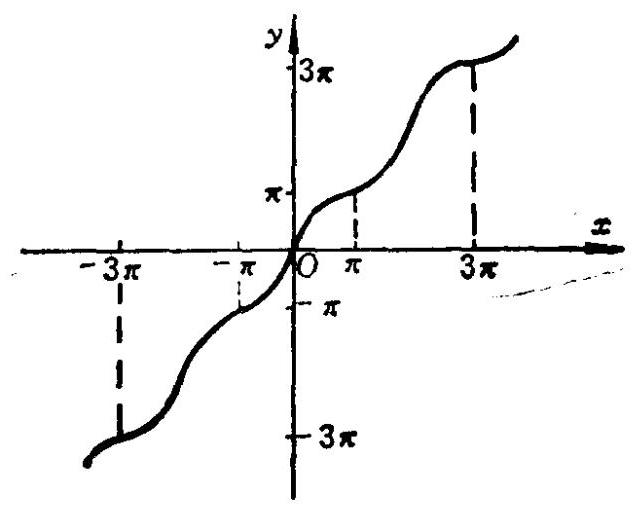
\includegraphics[max width=0.5\textwidth]{images/bo_d25ksc77aajc738obdgg_378_402_1440_632_505_0.jpg}
\end{center}
\hspace*{3em} 

图 71

\section*{4. 可化为有理分式求原函数的情形 II}

设 $f\left( {X,Y}\right)$ 是 $X,Y$ 的有理分式. 这里我们研究下述形式的原函数
$$I = \int f\left( {x,\sqrt[m]{\frac{{ax} + b}{{cx} + d}}}\right) {dx}$$

的计算问题. $\left( {a,b,c,d \in  \mathbf{R},m \in  \mathbf{N}}\right)$

作变换 $l = \sqrt[m]{\frac{{ax} + b}{{cx} + d}}$ ,于是
\begin{align*}
	&{t}^{m} = \frac{{ax} + b}{{cx} + d},x = \frac{d{t}^{m} - b}{-c{t}^{m} + a},\\
	&{x}^{\prime }\left( t\right)  = \frac{m\left( {{ad} - {bc}}\right) {t}^{m - 1}}{{\left( a - c{t}^{m}\right) }^{2}}.
\end{align*}

根据不定积分的变元替换法得到
\begin{align*}
	&I = \int f\left( {x,\sqrt[m]{\frac{{ax} + b}{{cx} + d}}}\right) {dx}\\
	&= \int f\left( {\frac{d{t}^{m} - b}{-c{t}^{m} + a},t}\right) \frac{m\left( {{ad} - {bc}}\right) {t}^{m - 1}}{{\left( a - c{t}^{m}\right) }^{2}}{dt}.
\end{align*}

因此 $I$ 的计算化为关于 $t$ 的有理分式的原函数的计算.

例 10 计算 $\int \frac{1}{\sqrt{x}}\frac{1}{\sqrt[3]{1 + \sqrt[4]{x}}}{dx}$ .

首先作变换 $y = \sqrt[4]{x}$ ,则 $x = {y}^{4},\sqrt{x} = {y}_{2}$ ,于是
\begin{align*}
	&\int \frac{1}{\sqrt{x}\sqrt[3]{1 + \sqrt[4]{x}}}{dx} = \int \frac{1}{{y}^{2}\sqrt[3]{1 + y}}{\left( {y}^{4}\right) }^{\prime }{dy}\\
	&\left( {y = \sqrt[4]{x}}\right)\\
	&= 4\int \frac{y}{\sqrt[3]{1 + y}}{dy}.
\end{align*}

再作变换 $t = \sqrt[3]{1 + y}$ ,则 $y = {t}^{3} - 1$ ,从而
\begin{align*}
	&\int \frac{y}{\sqrt[3]{1 + y}}{dy} = \int \frac{{t}^{3} - 1}{t}{\left( {t}^{3} - 1\right) }^{\prime }{dt}\;t = \sqrt[3]{1 + y}\\
	&= 3\int t\left( {t - 1}\right) {dt}\\
	&= \frac{3}{5}{t}^{5} - \frac{3}{2}{t}^{2} + C
\end{align*}

因此
\begin{align*}
	&\int \frac{1}{\sqrt{x\sqrt[3]{1 + \sqrt[4]{x}}}}{dx} = \frac{12}{5}{t}^{5} - 6{t}^{2} + C\;\left( {t = \sqrt[3]{1 + y}}\right)\\
	&=  - \frac{12}{5}\sqrt[3]{{\left( 1 + y\right) }^{5}} - 6\sqrt[3]{{\left( 1 + y\right) }^{2}}\\
	&+ C\;\left( {y = \sqrt[4]{x}}\right)\\
	&= \frac{12}{5}\sqrt[3]{{\left( 1 + \sqrt[4]{x}\right) }^{5}} - 6\sqrt[3]{{\left( 1 + \sqrt[4]{x}\right) }^{2}}\\
	&+ C\text{ . }
\end{align*}

\section*{5. 可化为有理分式求原函数的情形}

设 $f\left( {X,Y}\right)$ 是 $X,Y$ 的有理分式,我们来研究下述形式的原函数
$$I = \int f\left( {x,\sqrt{a{x}^{2} + {bx} + c}}\right) {dx}$$

的计算问题. $\left( {a,b,c \in  \mathbf{R},a \neq  0}\right)$

显然我们只能在集合 $E = \left\{  {x \in  \mathbf{R} \mid  a{x}^{2} + {bx} + c \geq  0}\right\}$ 上来讨论上述原函数的计算. 由于
\begin{align*}
	&a{x}^{2} + {bx} + c = a\left( {{x}^{2} + \frac{b}{a}x + \frac{c}{a}}\right)\\
	&= a{\left( x + \frac{b}{2a}\right) }^{2} + \frac{{4ac} - {b}^{2}}{4a},
\end{align*}

若令 $y = x + \frac{b}{2a}$ ,则
$$a{x}^{2} + {bx} + c = a{y}^{2} + \frac{{4ac} - {b}^{2}}{4a}.$$

所以不失一般性, 我们可以只讨论下述不定积分
$$I = \int f\left( {x,\sqrt{a{x}^{2} + c}}\right) {dx}\;\left( {a \neq  0,c \in  \mathbf{R}}\right) .$$

我们不妨假设 $c \neq  0$ ,否则上述不定积分就是 $x$ 的有理分式的不定积分. 这我们已经讨论过了.

下面对 $a,c$ 的符号分三种情况来讨论:
$$a > 0,c > 0;a > 0,c < 0;a < 0,c > 0.$$

1) $a > 0,c > 0$ :

因为 $f\left( {x,\sqrt{a{x}^{2} + c}}\right)  = f\left( {x,\sqrt{a\left( {{x}^{2} + \frac{c}{a}}\right) }}\right.$ . 所以我们可

作变换 $x = \sqrt{\frac{c}{a}}\operatorname{sh}\theta$ . 于是
\begin{align*}
	&I = \int f\left( {x,\sqrt{a{x}^{2} + c}}\right) {dx}\\
	&= \int f\left( {\sqrt{\frac{c}{a}}\operatorname{sh}\theta ,\sqrt{c}\operatorname{ch}\theta }\right) \sqrt{\frac{c}{a}}\operatorname{ch}{\theta d\theta }\\
	&\left( {\theta  = \operatorname{Argsh}\sqrt{\frac{a}{c}}x}\right)\\
	&= \int f\left( {\sqrt{\frac{c}{a}}\frac{{e}^{n} - {e}^{-\theta }}{2},\sqrt{c}\frac{{e}^{n} + {e}^{-\theta }}{2}}\right)  \cdot  \sqrt{\frac{c}{a}}\frac{{e}^{\theta } + {e}^{-\theta }}{2}{d\theta }\\
	&= \int f\left( {\sqrt{a}\frac{c}{a}\frac{{e}^{2\theta } - 1}{2{e}^{\theta }},\sqrt{c}\frac{{e}^{2\theta } + 1}{2{e}^{\theta }}}\right)  \cdot  \sqrt{a}\frac{c}{a}\frac{{e}^{2\theta } + 1}{2{e}^{2\theta }}{d\theta }\\
	&= \frac{1}{2}\sqrt{\frac{c}{a}}{\int }_{1}^{r}f\left( {\sqrt{\frac{c}{a}}\frac{{t}^{2} - 1}{2t},\sqrt{c}\frac{{t}^{2} + 1}{2t}}\right)  \cdot  \frac{{t}^{2} + 1}{{t}^{2}}{dt}\\
	&\left( {l = {e}^{\theta }}\right) \text{ . }
\end{align*}

因此 $I$ 的计算化为关于 $l$ 的有理分式的原函数的计算.

2) $a > 0,c < 0$ :

这时 $f\left( {x,\sqrt{a{x}^{2} + c}}\right)  = f\left( {x,\sqrt{a\left( {{x}^{2} - \frac{\left| c\right| }{a}}\right) }}\right)$ . 作变换 $x =$

$\sqrt{\frac{\left| c\right| }{a}}\operatorname{ch}\theta$ 则
\begin{align*}
	&I = \int f\left( {x,\sqrt{a{x}^{2} + c}}\right) {dx}\\
	&= \int f\left( {\sqrt{\frac{\left| c\right| }{a}}\operatorname{ch}\theta ,\sqrt{\left| c\right| }\operatorname{sh}\theta }\right) \sqrt{\frac{\left| c\right| }{a}}\operatorname{sh}{\theta d\theta }\\
	&\left( {\theta  = \operatorname{Argch}\sqrt{\frac{\sigma }{\left| c\right| }}x}\right)\\
	&= \frac{1}{2}\sqrt{\frac{\left| c\right| }{a}}\int f\left( {\sqrt{\frac{\left| c\right| }{a}}\frac{{t}^{2} + 1}{2t},\sqrt{\left| c\right| }\frac{{t}^{2} - 1}{2t}}\right) \frac{{t}^{2} - 1}{{t}^{2}}{dt}\\
	&\left( {t = {e}^{\theta }}\right) \text{ . }
\end{align*}

因此 $I$ 的计算也化为关于 $t$ 的有理分式的原函数的计算.

3) $a < 0,c > 0$ :

这时 $f\left( {x,\sqrt{a{x}^{2} + c}}\right)  = f\left( {x,\sqrt{\left| a\right| \left( {\frac{c}{\left| a\right| } - {x}^{2}}\right) }}\right)$ . 作变换 $x$

$= \sqrt{\frac{c}{\left| a\right| }}\sin \theta$ ,则
\begin{align*}
	&I = \int f\left( {x,\sqrt{a{x}^{2} + c}}\right) {dx}\\
	&= \int f\left( {\sqrt{\frac{c}{\left| a\right| }}\sin \theta ,\sqrt{c}\cos \theta }\right) \sqrt{\frac{c}{\left| a\right| }}\cos {\theta d\theta }\\
	&= \sqrt{\frac{c}{\left| a\right| }}\int f\left( {\sqrt{\frac{c}{\left| a\right| }}\sin \theta ,\sqrt{c}\cos \theta }\right) \cos {\theta d\theta }.
\end{align*}

因此 $I$ 的计算也最终化为有理公式的原函数的计算.

例 11 计算 $\int \sqrt{{x}^{2} + x + 1}{dx}$ .
\begin{align*}
	&I = \int \sqrt{{x}^{2} + x + 1}{dx}\\
	&= \int \sqrt{{\left( x + \frac{1}{2}\right) }^{2} + \frac{3}{4}}{dx}\\
	&= \int \sqrt{{y}^{2} + \frac{3}{4}}{dy}\;\left( {y = x + \frac{1}{2}}\right)\\
	&= \int \frac{\sqrt{3}}{2}\sqrt{{\operatorname{sh}}^{2}\theta  + 1}\frac{\sqrt{3}}{2}\operatorname{ch}{\theta d\theta }\\
	&\left( {y =  - \frac{\sqrt{3}}{2}\operatorname{sh}\theta }\right)\\
	&= \frac{3}{4}\int {\operatorname{ch}}^{2}{\theta d\theta }\\
	&= \frac{3}{4}\int {\left( \frac{{e}^{\theta } + {e}^{-\theta }}{2}\right) }^{2}{d\theta }\\
	&= \frac{3}{4}\int \frac{{\left( {e}^{2\theta } + 1\right) }^{2}}{4{e}^{3\theta }}{e}^{\theta }{d\theta }
\end{align*}
\begin{align*}
	&= \frac{3}{16}\int \frac{{t}^{4} + 2{t}^{2} + 1}{{t}^{3}}{dt}\;\left( {t = {e}^{\theta }}\right)\\
	&= \frac{3}{16}\left\lbrack  {\int {tdt} + 2\int \frac{1}{t}{dt} + \int \frac{1}{{t}^{3}}{dt}}\right\rbrack\\
	&= \frac{3}{32}{t}^{2} + \frac{3}{8}\log t - \frac{3}{{32}{t}^{2}} + C\\
	&= \frac{3}{32}\exp \left( {2\operatorname{Arg}\operatorname{sh}\frac{{2x} + 1}{\sqrt{3}}}\right)  + \frac{3}{8}\operatorname{Arg}\operatorname{sh}\frac{{2x} + 1}{\sqrt{3}}\\
	&- \frac{3}{32}\exp \left( {-2\mathrm{{Arg}}\operatorname{sh}\frac{{2x} + 1}{\sqrt{3}}}\right)  + C.
\end{align*}

例 12 计算 $\int \frac{1}{\sqrt{{a}^{2} - {x}^{2}}}{dx}\;\left( {a > 0}\right)$ .

作变换 $x = a\sin \theta ,\theta  \in  \rbrack  - \frac{\pi }{2},\frac{\pi }{2}\lbrack$ ,则
\begin{align*}
	&\int \frac{1}{\sqrt{{a}^{2} - {x}^{2}}}{dx} = \int \frac{1}{\sqrt{{a}^{2} - {a}^{2}{\sin }^{2}\theta }}{\left( a\sin \theta \right) }^{\prime }{d\theta }\\
	&\left( {\theta  = \arcsin \frac{x}{a}}\right)\\
	&= \int \frac{a\cos \theta }{a\cos \theta }{d\theta }\\
	&= \int {d\theta }\\
	&= \theta  + C\\
	&= \arcsin \frac{x}{a} + C\text{ . }
\end{align*}

\section*{习 题}

1. 计算下列各有理分式的原函数:

1) $\int \frac{1}{\left( {x - a}\right) \left( {x - b}\right) \left( {x - c}\right) }{dx}$ ,

2) $\int \frac{{x}^{3} + 2{x}^{2} + {2x} + 1}{x\left( {{x}^{2} + 1}\right) }{dx}$ ,

3) $\int \frac{1}{{x}^{4} - 1}{dx}$ ,

4) $\int \frac{{x}^{2}}{{\left( 1 + {x}^{2}\right) }^{2}}{dx}$ ,

5) $\int \frac{1}{\left( {{x}^{2} + {2x} + 2}\right) \left( {{x}^{2} + {2x} + 5}\right) }{dx}$ ,

6) $\int \frac{1}{{x}^{4} + {x}^{2} + 1}{dx}$ ,

7) $\int \frac{{x}^{2}}{{\left( {x}^{2} + x + 1\right) }^{2}}{dx}$ ,

8) $\int \frac{{x}^{2} + {x}^{2} - 1}{{\left( x - 2\right) }^{3}}{dx}$ ,

9) $\int \frac{{x}^{5} + 1}{{\left( {x}^{2} + x + 1\right) }^{2}} - {dx}$ ,

10) $\int \frac{1}{{\left( x + 1\right) }^{7} - {x}^{7} - 1}{dx}$ .

2. 设
$$f\left( x\right)  = \frac{a{x}^{2} + {bx} + c}{{\left( {x}^{2} + {k}^{2}\right) }^{2}}\;\left( {a,b,c,k \in  \mathrm{R},a \neq  0,k \neq  0}\right) .$$

试问常数 $a\text{ 、 }b\text{ 、 }c$ 取何值时,可以保证 $f$ 的原函数 $\int f\left( x\right) {dx}$ 是一个有理分式?

3. 计算下列各原函数:

1) $\int {\sin }^{2}x{\cos }^{3}{xdx}$ ,

2) $\int \frac{1}{{\sin }^{2}x{\cos }^{4}x}{dx}$ ,

3) $\int \frac{\cos x}{{\left( 1 - \cos x\right) }^{2}}{dx}$ ,

4) $\int \frac{\sin x}{{\left( 1 - \cos x\right) }^{n + 1}}{dx}\;\left( {n \in  N}\right)$ ,

5) $\int \frac{\cos x}{1 + \cos x}{dx}$ ,

6) $\int \frac{{\cos }^{2}x - {\sin }^{2}x}{{\cos }^{4}x + {\sin }^{4}x}{dx}$ ,

7) $\int \frac{{\cos }^{3}x}{{\sin }^{2}x + \sin x + 1}{dx}$ ,

8) $\int \frac{\left( {1 + {\operatorname{tg}}^{2}x}\right) {\sin }^{3}x}{{\cos }^{2}x + 2\cos x + 2}{dx}$ ,

9) $\int \frac{{\cos }^{2}x}{\left( {\sin x - 2}\right) \left( {\sin x + 2}\right) }{dx}$ ,

10) $\int \frac{1}{2\sin x - \cos x + 5}{dx}$ .

4. 计算下列各原函数

1) $\int \frac{1}{1 + \sqrt{x}}{dx}$ ,

2) $\int \frac{\sqrt[3]{1 + \sqrt[4]{x}}}{\sqrt{x}}{dx}$ ,

3) $\int \frac{\sqrt{x} - 1}{\sqrt[3]{x} + 1}{dx}$ ,

4) $\int \frac{1 - \sqrt{x + 1}}{1 + \sqrt[3]{x + 1}}{dx}$ ,

5) $\int \frac{1}{\sqrt{x}{\left( 1 + \sqrt[4]{x}\right) }^{3}}{dx}$ ,

6) $\int \frac{\sqrt{x - 1} + 2}{\sqrt{{\left( x - 1\right) }^{2}} - \left( {x - 1}\right) }{dx}$ ,

7) $\int \frac{1}{x}\sqrt{\frac{1 + x}{x}}{dx}$ ,

8) $\int \frac{{2x} + 1}{{x}^{2}\sqrt{{2x} + 1}}{dx}$ ,

9) $\int \frac{1}{\left( {2 + x}\right) \sqrt{x + 1}}{dx}$ ,

10) $\int \frac{1}{\sqrt[3]{\left( {x - 1}\right) {\left( x + 1\right) }^{2}}}{dx}$ .

5. 计算下列各原函数:

1) $\int \frac{1}{\sqrt{{x}^{2} + {2x} + 5}}{dx}$ ,

2) $\int \frac{{3x} + 2}{\left( {x + 1}\right) \sqrt{{x}^{2} + {3x} + 3}}{dx}$ ,

3) $\int \frac{\sqrt{{x}^{2} + x + 1}}{{2x} + 1}{dx}$ ,

4) $\int \frac{{x}^{2} - x + 1}{x\sqrt{{x}^{2} + {2x} + 2}}{dx}$ ,

5) $\int \frac{{5x} - 3}{\sqrt{2{x}^{2} + {8x} + 1}}{dx}$ ,

6) $\int \frac{x + 1}{\sqrt{-{x}^{2} + {6x} - 8}}{dx}$ ,

7) $\int \frac{1}{\left( {x - 1}\right) \sqrt{-{x}^{2} + {2x} + 3}}{dx}$ ,

8) $\int {x}^{2}\sqrt{1 - {x}^{2}}{dx}$ ,

g) $\int \frac{1}{x + \sqrt{{x}^{2} - x + 1}}{dx}$ ,

10) $\int \sqrt{{e}^{2x} + 2{e}^{x} + 2}{dx}$ .

6. 计算下列各原函数:

1) $\int \frac{1 - \operatorname{tg}x}{1 + \operatorname{tg}x}{dx}$ ,

2) $\int \frac{\sin \sqrt{x} + \cos \sqrt{x}}{\sqrt{x}{\sin }^{2}\sqrt{x}}{dx}$ ,

3) $\int \frac{x}{{\operatorname{ch}}^{2}x}{dx}$ ,

4) $\int \frac{\operatorname{ch}\sqrt{1 + x}}{\sqrt{1 + x}}{dx}$ ,

5) $\int \frac{1}{1 + {\mathrm{{ch}}}^{2}x}{dx}$ ,

6) $\int \frac{1}{\operatorname{sh}x + 2\operatorname{ch}x}{dx}$ ,

7) $\int \frac{{\operatorname{ch}}^{3}x}{1 + \operatorname{sh}x}{dx}$ ,

8) $\int {\operatorname{sh}}^{4}{xdx}$ ,

9) $\int \sqrt{\operatorname{th}x}{dx}$ ,

10) $\int {\operatorname{cth}}^{2}{xdx}$ .

